\section{Introduction to the Chapter}
\label{sec:chapter_intro}

This chapter presents the numerical results obtained with the \texttt{radpattern} simulation framework. The chapter is organized from a macroscopic warm-vapour reference geometry to a compact boundary-dominated cell, and finally to the contactless ultracold regime.

The main observable used throughout the chapter is the normalized retrievable-mode coupling,
\begin{equation}
    \eta(t)
    =
    \frac{P_{\mathrm{fib}}(t)}{P_{\mathrm{tot}}(0)} ,
    \label{eq:eta_pfibt_ptot0}
\end{equation}
where $P_{\mathrm{fib}}(t)$ is the power coupled into the target fibre mode at time $t$, and $P_{\mathrm{tot}}(0)$ is the initial total emitted power.

The coherent fibre-coupled amplitude is evaluated from the ensemble as
\begin{equation}
    A_{\mathrm{fib}}(t)
    \propto
    \sum_{j}
    w_j(t)
    e^{i\phi_j(t)}
    u_{\mathrm{fib}}^*\!\left(\mathbf r_j(t)\right),
    \label{eq:fiber_mode_sum}
\end{equation}
where $w_j(t)$ is the atomic weight, $\phi_j(t)$ is the accumulated spin-wave phase, $u_{\mathrm{fib}}$ is the target optical mode, and $\mathbf r_j(t)$ is the position of atom $j$.

\begin{figure}[htbp]
    \centering
    \includegraphics[width=0.85\textwidth]{Figures/spinwave_retrieval_concept.jpeg}
    \caption{Temporary caption: Schematic of the stored spin wave and the retrieved fibre-coupled mode. The figure should define the signal beam, control beam, ensemble, spin-wave phase, and target output mode.}
    \label{fig:chapter_concept_spinwave_retrieval}
\end{figure}

\section{Macroscopic Validation and Sensitivity Checks}
\label{sec:macroscopic_validation}

This section uses a ${}^{133}\mathrm{Cs}$ warm-vapour reference geometry based on a long cylindrical cell. The baseline geometry is a $\SI{75}{\milli\metre}$ long and $\SI{4}{\milli\metre}$ diameter cell operated near $\SI{75}{\celsius}$, with $N_2$ buffer gas and focused signal and control beams.

\begin{figure}[htbp]
    \centering
    \includegraphics[width=0.85\textwidth]{Figures/jutisz_reference_geometry.jpeg}
    \caption{Temporary caption: Reference warm-vapour geometry used for validation. The figure should show the $\SI{75}{\milli\metre}$ by $\SI{4}{\milli\metre}$ cylindrical cell, the signal and control beams, the buffer gas, and the fibre-coupled output mode.}
    \label{fig:jutisz_reference_geometry}
\end{figure}

\subsection{Directional Emission and Coherent Radiative Profiles}
\label{subsec:directional_emission}

The first validation step is to verify that the stored spin wave produces directional collective emission. The simulation treats the ensemble as a set of phased microscopic emitters, whose far-field interference determines the retrieved optical mode.

\begin{figure}[htbp]
    \centering
    \begin{minipage}[t]{0.48\textwidth}
        \centering
        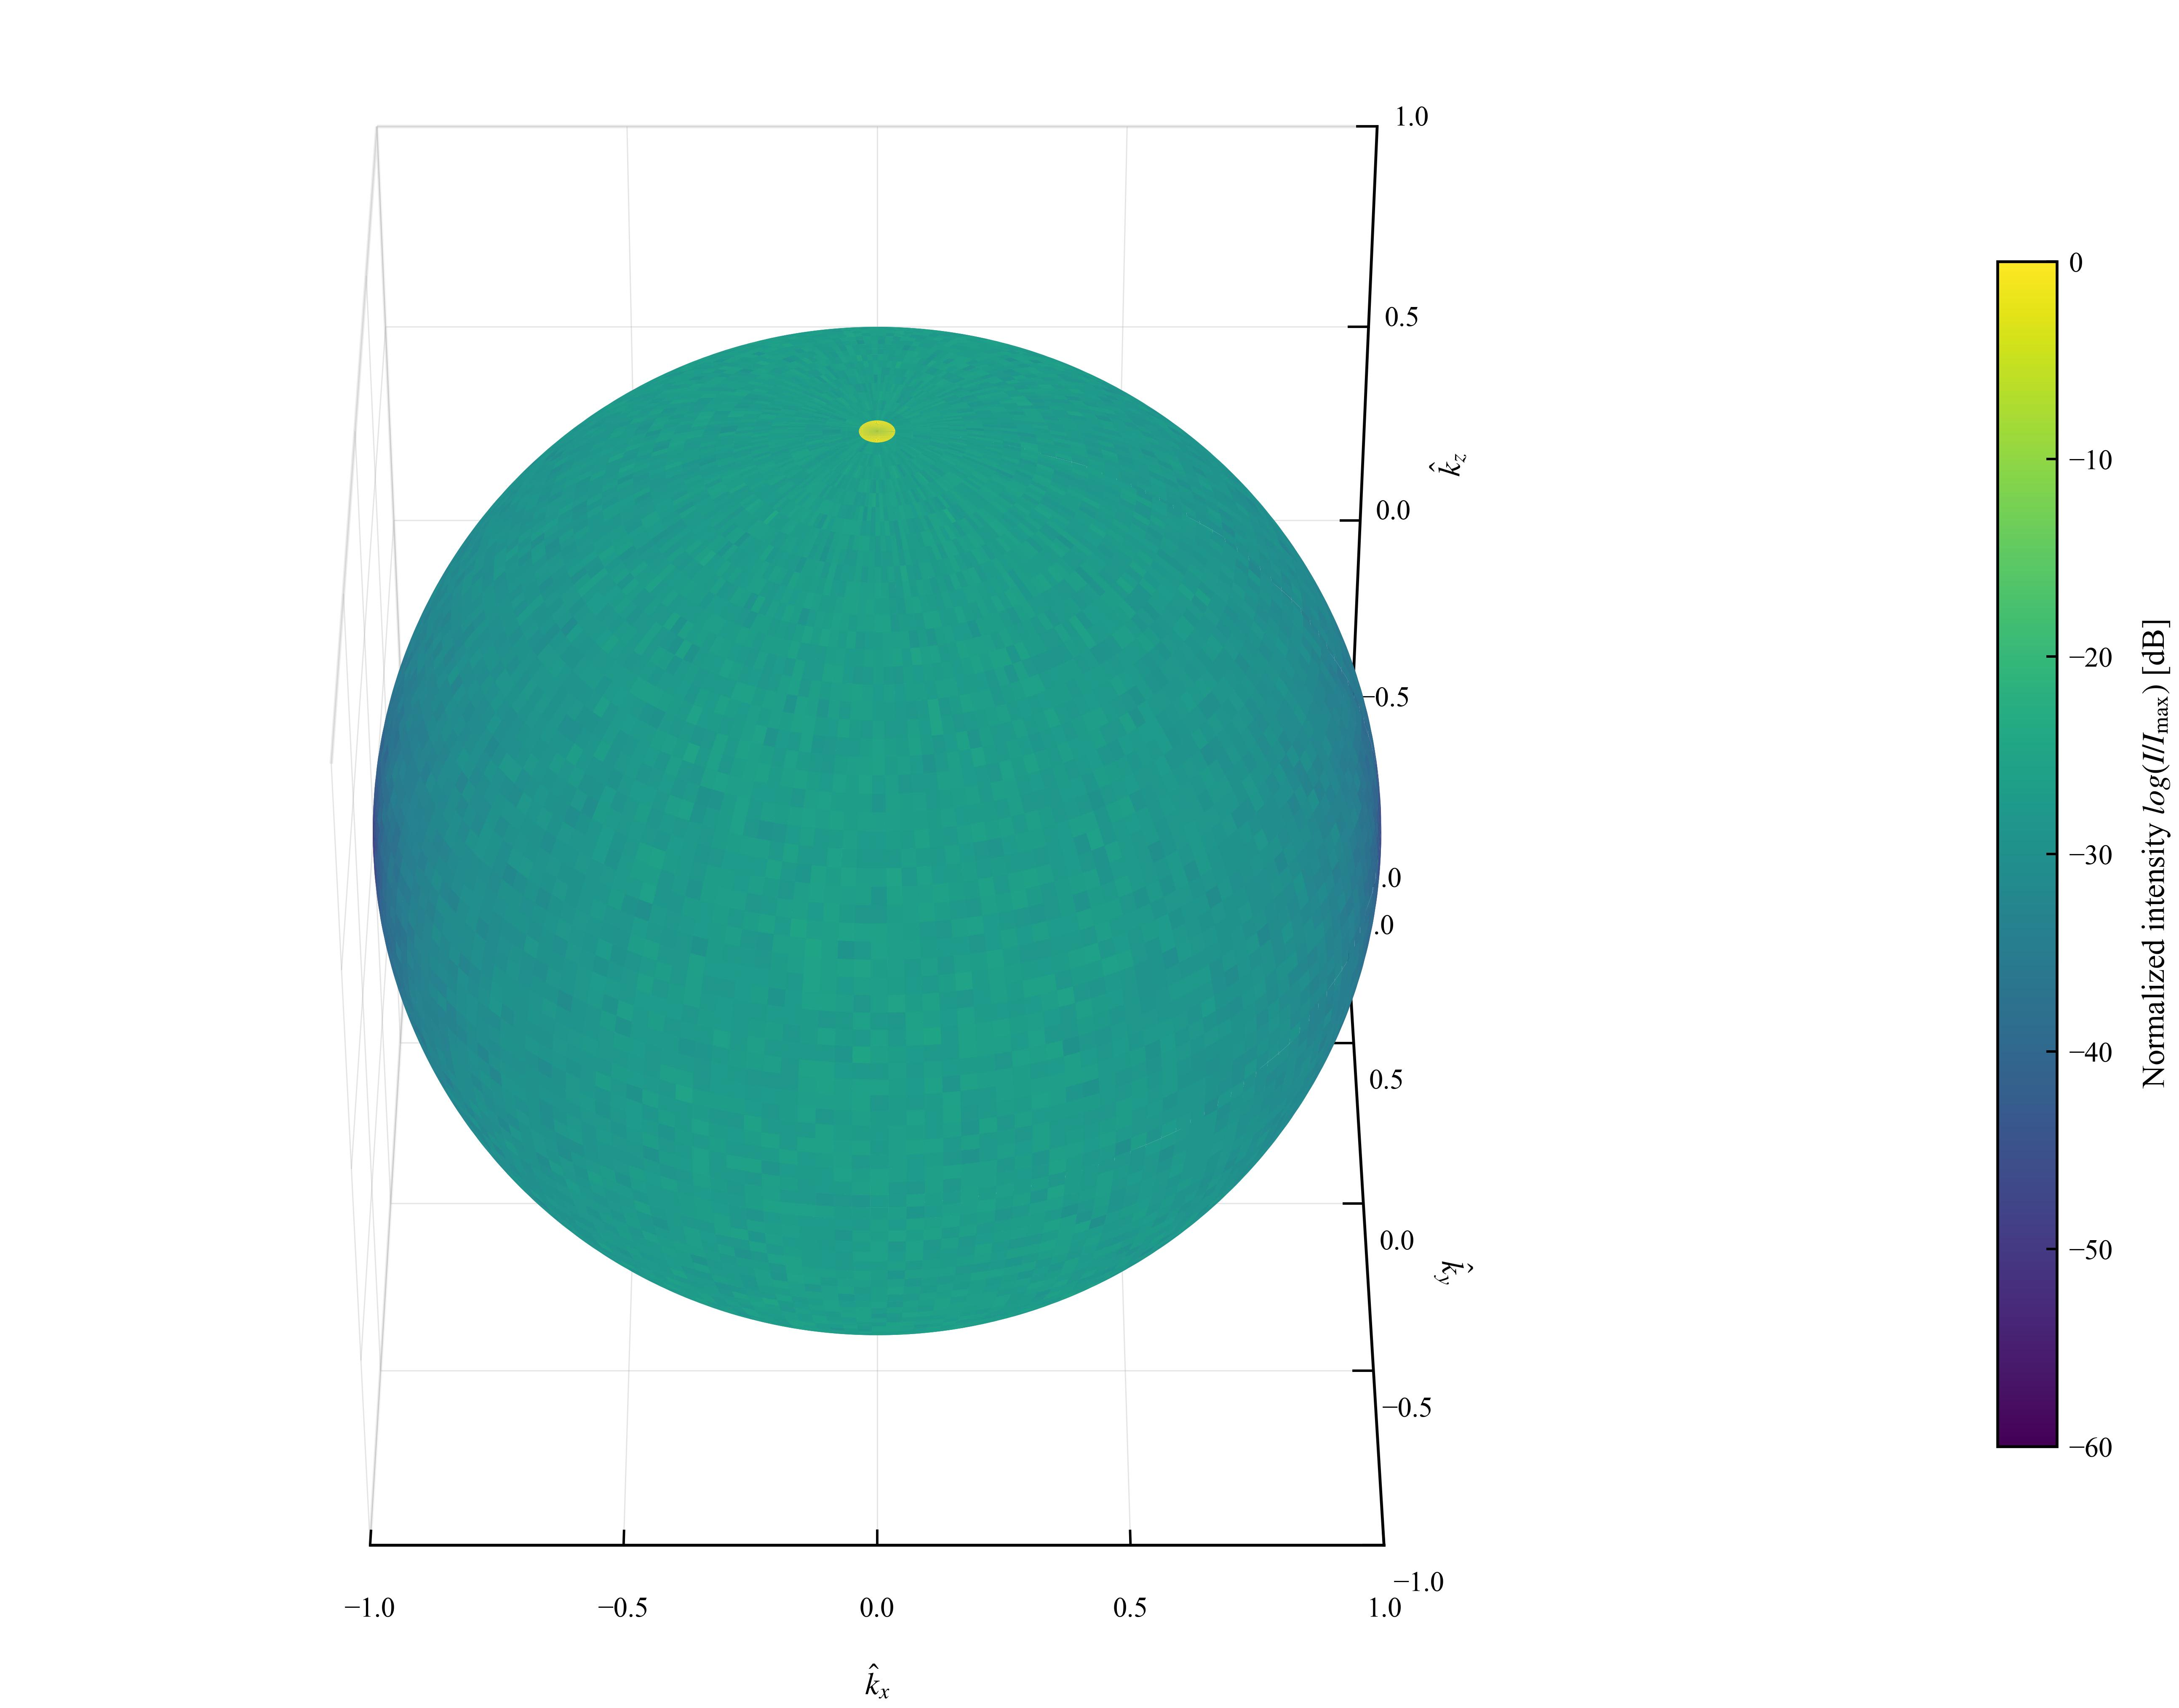
\includegraphics[width=\textwidth]{Figures/far_field_angular_emission_profile.jpeg}
    \end{minipage}
    \hfill
    \begin{minipage}[t]{0.48\textwidth}
        \centering
        \includegraphics[width=\textwidth]{Figures/weighted_atom_cloud_distribution.jpeg}
    \end{minipage}
    \caption{Temporary caption: Left: far-field angular emission profile from the collective spin-wave distribution. Right: three-dimensional atom cloud with normalized atomic weights $|w|_{\mathrm{norm}}$. Together, these plots show that the retrieved signal is a directional coherent-emission mode rather than an incoherent atom-number signal.}
    \label{fig:directional_emission_cloud_weights}
\end{figure}

\subsection{Convergence and Statistical Stability}
\label{subsec:mc_convergence}

Monte Carlo convergence is checked by comparing individual stochastic realizations with the ensemble-averaged coupling curve. This verifies that the simulated decay is not dominated by sampling noise or by a small number of rare trajectories.

\begin{figure}[htbp]
    \centering
    \includegraphics[width=0.78\textwidth]{Figures/mc_convergence_realizations.jpeg}
    \caption{Temporary caption: Monte Carlo convergence check. Thin curves show individual realizations, while the thick curve shows the ensemble average. The figure should demonstrate that the long-time decay and plateau features are statistically stable.}
    \label{fig:mc_convergence}
\end{figure}

\subsection{Gas-Phase Transport and Spatial Escape}
\label{subsec:pressure_scans}

The buffer gas pressure controls the diffusion coefficient and therefore the time scale over which atoms leave the high-overlap optical mode. Pressure scans are used to validate the gas-phase transport model.

\begin{figure}[htbp]
    \centering
    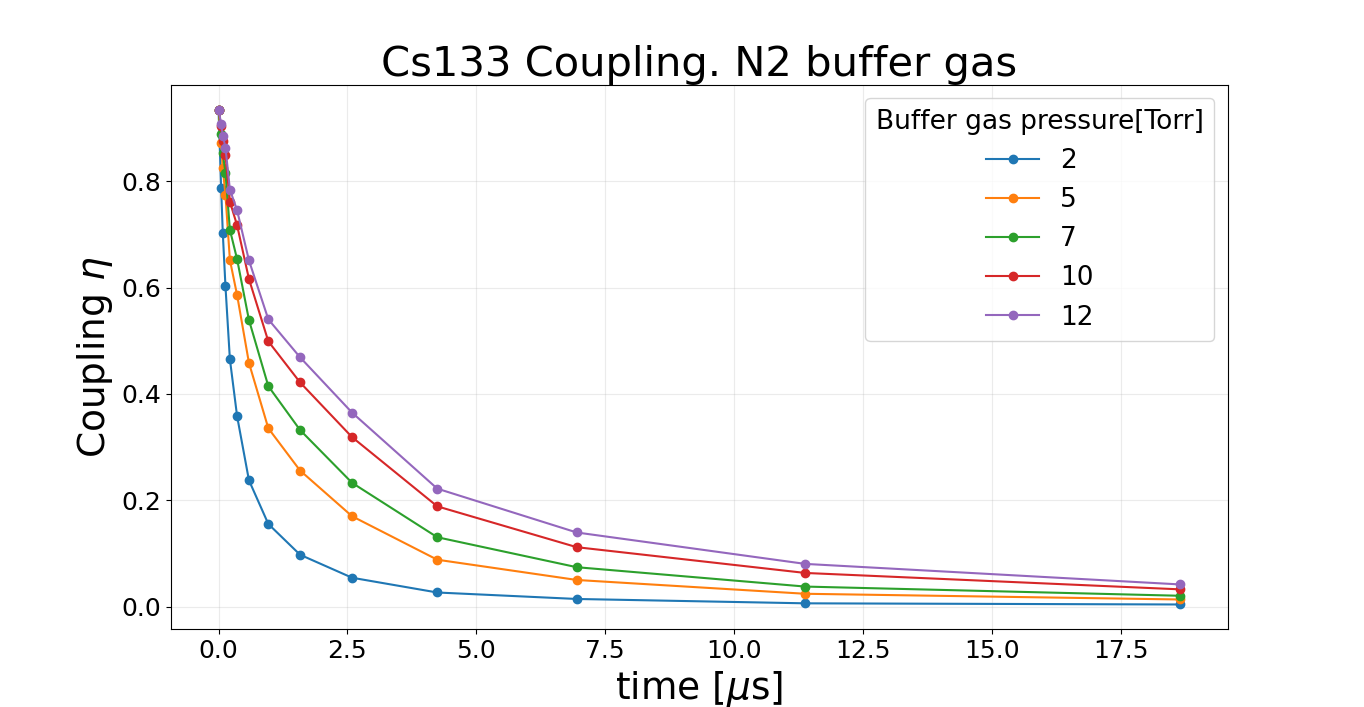
\includegraphics[width=0.78\textwidth]{Figures/pressure_scan_coupling_decay.jpeg}
    \caption{Temporary caption: Coupling decay $\eta(t)$ for different $N_2$ buffer gas pressures in the $\SI{75}{\milli\metre}$ reference cell. Higher pressure reduces diffusion and slows the loss of fibre-mode overlap.}
    \label{fig:pressure_scan_eta}
\end{figure}

\begin{figure}[htbp]
    \centering
    \includegraphics[width=0.72\textwidth]{Figures/pressure_scan_decay_time.jpeg}
    \caption{Temporary caption: Extracted characteristic decay time $\tau_{\eta}$ as a function of $N_2$ buffer gas pressure. This plot summarizes the pressure dependence of the retrievable-mode lifetime.}
    \label{fig:pressure_scan_tau}
\end{figure}

\subsection{Beam-Size Dependence}
\label{subsec:beam_size_dependence}

The optical beam dimensions set the spatial region over which atoms contribute efficiently to the retrieved mode. Larger beams are expected to reduce diffusion-driven escape from the optical mode, while smaller beams increase sensitivity to atomic motion.

\begin{figure}[htbp]
    \centering
    \includegraphics[width=0.78\textwidth]{Figures/beam_size_coupling_decay.jpeg}
    \caption{Temporary caption: Coupling decay $\eta(t)$ for different signal or control beam diameters. Larger beams produce slower mode-overlap decay because atoms remain inside the optically weighted region for longer times.}
    \label{fig:beam_size_eta}
\end{figure}

\begin{figure}[htbp]
    \centering
    \includegraphics[width=0.72\textwidth]{Figures/beam_size_decay_time.jpeg}
    \caption{Temporary caption: Extracted decay time $\tau_{\eta}$ as a function of beam diameter. This plot summarizes the sensitivity of the retrievable-mode lifetime to the transverse optical mode size.}
    \label{fig:beam_size_tau}
\end{figure}

\section{Phase-Gradient and Vector Perturbations in Bulk Media}
\label{sec:phase_gradient_perturbations}

This section isolates mechanisms that degrade the coherent sum without requiring atoms to collide with a physical boundary. The two main perturbations are geometric phase mismatch from beam misalignment and Zeeman dephasing from magnetic-field gradients.

\subsection{Geometric Phase Mismatch from Control-Beam Angle}
\label{subsec:control_beam_angle}

A change in the control-beam direction changes the phase-matching condition. The relevant wave-vector mismatch is
\begin{equation}
    \Delta \mathbf{k}
    =
    \mathbf{k}_{\mathrm{sig}}
    -
    \mathbf{k}_{\mathrm{c}} .
    \label{eq:delta_k_angle}
\end{equation}
Small milliradian angular offsets impose a transverse phase gradient across the ensemble and reduce the constructive interference into the target mode.

\begin{figure}[htbp]
    \centering
    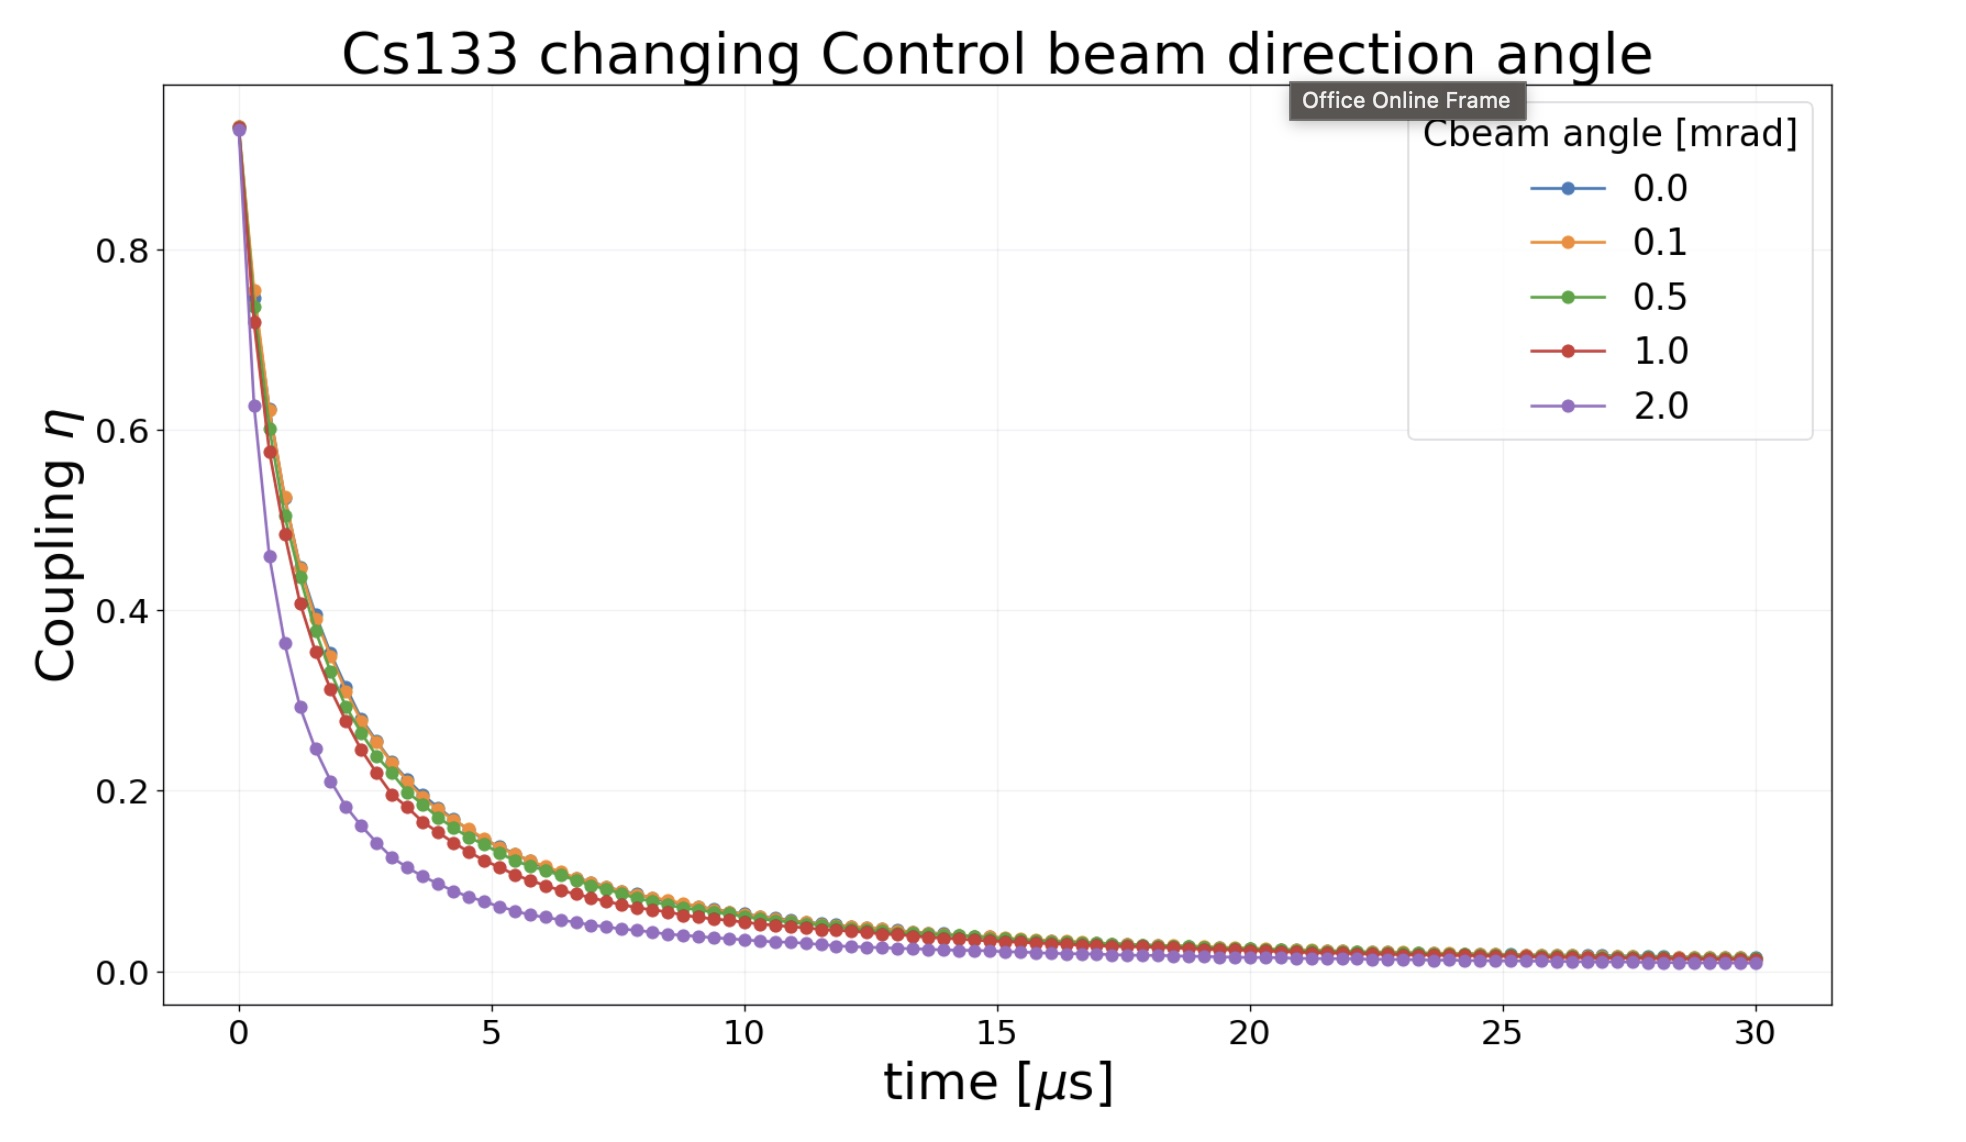
\includegraphics[width=0.78\textwidth]{Figures/control_beam_angle_scan.jpeg}
    \caption{Temporary caption: Coupling decay $\eta(t)$ for different control-beam angular offsets. The scan should include milliradian-scale angles and show the degradation of phase-matched retrieval with increasing angular mismatch.}
    \label{fig:control_angle_scan}
\end{figure}

\begin{figure}[htbp]
    \centering
    \includegraphics[width=0.72\textwidth]{Figures/control_beam_angle_tolerance_summary.jpeg}
    \caption{Temporary caption: Coupling at a fixed storage time, or fitted decay time $\tau_{\eta}$, as a function of control-beam angle. This plot summarizes the angular tolerance of the retrieval geometry.}
    \label{fig:control_angle_summary}
\end{figure}

\subsection{Zeeman Scrambling from Magnetic-Field Gradients}
\label{subsec:magnetic_gradient}

A uniform magnetic field produces only a global phase. By contrast, a magnetic-field gradient produces position-dependent spin-wave precession,
\begin{equation}
    \phi_j(t)
    =
    \phi_j(0)
    -
    \omega_{sg}\!\left(\mathbf r_j\right)t ,
    \label{eq:position_dependent_phase}
\end{equation}
which reduces the coherent fibre-coupled amplitude.

\begin{figure}[htbp]
    \centering
    \begin{minipage}[t]{0.48\textwidth}
        \centering
        \includegraphics[width=\textwidth]{Figures/cs_magnetic_gradient_scan.jpeg}
    \end{minipage}
    \hfill
    \begin{minipage}[t]{0.48\textwidth}
        \centering
        \includegraphics[width=\textwidth]{Figures/rb_magnetic_gradient_scan.jpeg}
    \end{minipage}
    \caption{Temporary caption: Magnetic-field-gradient scans for Cs and Rb configurations. The curves show how spatially varying Zeeman shifts dephase the spin wave and reduce the phase-matched fibre coupling.}
    \label{fig:magnetic_gradient_cs_rb}
\end{figure}

\section{The Compact-Cell Boundary Regime}
\label{sec:compact_cell_boundary_regime}

The validated model is next applied to a compact ${}^{133}\mathrm{Cs}$ cell with diameter $\SI{1}{\milli\metre}$ and length $\SI{1}{\centi\metre}$. The control beam has diameter $\SI{0.8}{\milli\metre}$, and the signal beam has diameter $\SI{0.3}{\milli\metre}$. In this geometry, the control beam occupies a large fraction of the available transverse cell size, so wall interactions and boundary reflections can no longer be treated as negligible.

\begin{figure}[htbp]
    \centering
    \includegraphics[width=0.78\textwidth]{Figures/compact_cell_geometry.jpeg}
    \caption{Temporary caption: Compact-cell geometry. The figure should show the $\SI{1}{\milli\metre}$ diameter cell, the $\SI{1}{\centi\metre}$ length, the $\SI{0.8}{\milli\metre}$ control beam, the $\SI{0.3}{\milli\metre}$ signal beam, and the proximity of the optical modes to the walls.}
    \label{fig:compact_cell_geometry}
\end{figure}

\subsection{Breakdown of a Single-Exponential Lifetime}
\label{subsec:single_exponential_breakdown}

In the compact geometry, the coupling decay can contain a fast initial loss followed by a slow tail or plateau. This occurs because atoms can reflect from the boundaries and re-enter the high-overlap region. Therefore, a single exponential form,
\begin{equation}
    \eta(t)
    =
    \eta_0 e^{-t/\tau},
    \label{eq:single_exp_fit}
\end{equation}
may not be a physically complete description of the compact-cell dynamics.

\begin{figure}[htbp]
    \centering
    \includegraphics[width=0.78\textwidth]{Figures/compact_cell_long_time_decay.jpeg}
    \caption{Temporary caption: Long-time coupling decay in the compact $\SI{1}{\milli\metre}$ cell. The plot should highlight the non-single-exponential structure, including the initial decay, slow tail, and possible plateau produced by reflection and re-entry.}
    \label{fig:compact_cell_long_time_decay}
\end{figure}

\subsection{Surface Chemistry Abstraction: Coating and Wall-Bounce Scans}
\label{subsec:coating_wall_bounce_scans}

Wall depolarization is represented by an effective survival parameter $N_{\text{b}}$, defined as the average number of wall collisions an atom can undergo before losing its spin-wave coherence. The scan covers poor wall survival up to nearly ideal anti-relaxation behaviour, for example once $N_{\text{b}}\sim \num{1e3}\text{ to }\num{1e4}$ and above.

\begin{figure}[htbp]
    \centering
    \includegraphics[width=0.78\textwidth]{Figures/compact_cell_wall_survival_decay.jpeg}
    \caption{Temporary caption: Compact-cell coupling decay $\eta(t)$ for different wall-survival parameters $N_{\text{b}}$. The scan should include values from $N_{\text{b}}=\num{1e3}$ to $N_{\text{b}}=\num{1e12}$, showing the transition from wall-limited decay to a geometry- or diffusion-limited plateau.}
    \label{fig:compact_cell_nbounces_eta}
\end{figure}

\begin{figure}[htbp]
    \centering
    \includegraphics[width=0.72\textwidth]{Figures/compact_cell_wall_survival_design.jpeg}
    \caption{Temporary caption: Design summary plot showing $\eta(t_{\mathrm{target}})$ or $\tau_{\eta}$ as a function of $N_{\text{b}}$. The expected behaviour is a strong improvement at low $N_{\text{b}}$, followed by saturation once wall relaxation is no longer the dominant limitation.}
    \label{fig:compact_cell_nbounces_design}
\end{figure}

\subsection{Beam Size, Coating Quality, and Buffer Gas Coupling}
\label{subsec:beam_coating_pressure_tradeoff}

The compact geometry couples several design parameters. Increasing the beam size improves mode-overlap lifetime but also brings the optical mode closer to the walls. Increasing buffer gas pressure slows diffusion, while improving the coating increases survival during wall encounters. These variables should therefore be interpreted together.

\begin{figure}[htbp]
    \centering
    \includegraphics[width=0.78\textwidth]{Figures/compact_cell_joint_design_map.jpeg}
    \caption{Temporary caption: Joint design map for the compact cell. Possible axes include beam diameter and $N_{\text{b}}$, or buffer gas pressure and $N_{\text{b}}$, with colour representing $\eta(t_{\mathrm{target}})$ or $\tau_{\eta}$.}
    \label{fig:compact_cell_design_map}
\end{figure}

\section{Contactless Confinement: The Ultracold BEC Regime}
\label{sec:bec_regime}

The ultracold regime provides an alternative limit in which physical wall collisions are removed. Instead of wall-limited diffusion, the relevant spatial evolution comes from the initial trapped density distribution, ballistic expansion, gravitational sag, and trap-induced motion.

\subsection{Mapping the Trap Profile}
\label{subsec:bec_trap_profile}

The initial density distribution is no longer uniform inside a cylinder. Instead, the atom cloud follows a trapped density profile, such as a Gaussian or Thomas-Fermi distribution. This modifies the initial spatial overlap with the optical mode.

\begin{figure}[htbp]
    \centering
    \begin{minipage}[t]{0.48\textwidth}
        \centering
        \includegraphics[width=\textwidth]{Figures/bec_density_distribution.jpeg}
    \end{minipage}
    \hfill
    \begin{minipage}[t]{0.48\textwidth}
        \centering
        \includegraphics[width=\textwidth]{Figures/bec_weight_distribution.jpeg}
    \end{minipage}
    \caption{Temporary caption: Ultracold cloud initialization. Left: three-dimensional density distribution of the trapped cloud. Right: spatial distribution of the normalized atomic weights $|w|_{\mathrm{norm}}$ relative to the target optical mode.}
    \label{fig:bec_density_weights}
\end{figure}

\subsection{Free Expansion and Trap-Induced Drift}
\label{subsec:bec_motion_profiles}

If the trap is released, the cloud expands ballistically. The characteristic thermal velocity $v_{\text{th}}$ produces a time-dependent spatial footprint, which modifies the spin-wave overlap with the fibre mode. If the trap remains on, the dominant motion may instead come from residual drift, gravitational sag, or trap oscillations.

\begin{figure}[htbp]
    \centering
    \includegraphics[width=0.78\textwidth]{Figures/bec_motion_decay.jpeg}
    \caption{Temporary caption: Coupling decay $\eta(t)$ for different ultracold motion models, such as released ballistic expansion and trapped-cloud drift. The comparison isolates spatial overlap loss without wall collisions.}
    \label{fig:bec_motion_eta}
\end{figure}

\section{Engineering Synthesis: Comparing the Two Extremes}
\label{sec:engineering_synthesis}

The warm compact cell and ultracold cloud represent two limiting regimes of spatial-mode degradation. The compact warm cell is boundary dominated, while the ultracold cloud is contactless but sensitive to expansion and drift.

\subsection{Collision-Dominated and Ballistic Regimes}
\label{subsec:collision_vs_ballistic}

The decay profiles from both regimes can be compared directly. A compact coated cell can show non-single-exponential decay and long-time plateaus due to reflection and re-entry. An ultracold released cloud is expected to show smoother overlap loss associated with ballistic expansion or drift.

\begin{figure}[htbp]
    \centering
    \includegraphics[width=0.78\textwidth]{Figures/warm_compact_vs_bec_decay.jpeg}
    \caption{Temporary caption: Direct comparison of representative coupling decays from the compact warm-vapour cell and the ultracold cloud. The figure should emphasize the difference between boundary-mediated re-entry and smooth ballistic or trap-induced spatial loss.}
    \label{fig:warm_compact_vs_bec_decay}
\end{figure}

\subsection{Pressure, Coating, Temperature, and Trap Parameters}
\label{subsec:parameter_synthesis}

The final comparison summarizes the controlling design parameters in each regime. Warm-vapour operation depends on buffer gas pressure, temperature, beam size, and wall-survival parameter $N_{\text{b}}$. Ultracold operation depends on trap frequencies, release time, temperature, cloud size, and spatial drift.

\begin{figure}[htbp]
    \centering
    \includegraphics[width=0.82\textwidth]{Figures/warm_vapor_bec_parameter_synthesis.jpeg}
    \caption{Temporary caption: Summary of the dominant design parameters for warm-vapour compact cells and ultracold clouds. The plot may be implemented as a table-style figure, mechanism map, or bar chart comparing characteristic decay times.}
    \label{fig:parameter_synthesis}
\end{figure}

\section{Chapter Summary}
\label{sec:simulation_results_summary}

This chapter has organized the simulation results into three regimes: a macroscopic warm-vapour reference cell, a compact boundary-dominated warm-vapour cell, and a contactless ultracold cloud. The common metric throughout is the decay of the retrievable spatial mode, quantified by $P_{\mathrm{fib}}(t)/P_{\mathrm{tot}}(0)$. The results separate diffusion-driven loss, phase-gradient dephasing, wall-induced relaxation, and contactless expansion as distinct mechanisms controlling the usable memory lifetime.



\chapter{========}%
\label{sec:========}

\chapter{Simulation Results}
\label{chap:simulation_results}

\section{Validation Strategy and Reference Geometry}
\label{sec:results_validation_strategy}

The first purpose of the simulations is not to claim a new storage protocol, but to verify that the numerical model reproduces the physical behaviour expected from a collective spin-wave memory. The relevant observable throughout this chapter is the retrieved mode overlap, written as
\begin{equation}
    \mathcal{R}_{\mathrm{fib}}(t)
    =
    \frac{P_{\mathrm{fib}}(t)}
    {P_{\text{tot}}(0)},
    \label{eq:results_normalized_retrieval}
\end{equation}
where \(P_{\mathrm{fib}}(t)\) is the power coupled into the target fibre mode after a storage time \(t\), and \(P_{\text{tot}}(0)\) is the total emitted power at zero storage time. This normalization is used because the simulations are designed to follow the decay of the retrievable collective mode, rather than the absolute optical efficiency of a full EIT memory.

The reference geometry is based on the standalone caesium warm-vapour memory reported by Jutisz \emph{et al.}~\cite{Smqms_JutiszEtAl_2025}. The simulated cell is a long cylindrical \({}^{133}\mathrm{Cs}\) vapour cell with length \(\SI{75}{\milli\metre}\) and diameter \(\SI{4}{\milli\metre}\), operated near \(\SI{75}{\celsius}\) with nitrogen buffer gas. The signal and control fields are modelled as Gaussian beams. In this geometry, the optical mode occupies only a small fraction of the full transverse cell area. The simulation can therefore focus on the atoms that significantly overlap with the signal and control modes, instead of sampling the entire vapour volume with equal resolution.

\begin{figure}[htbp]
    \centering
    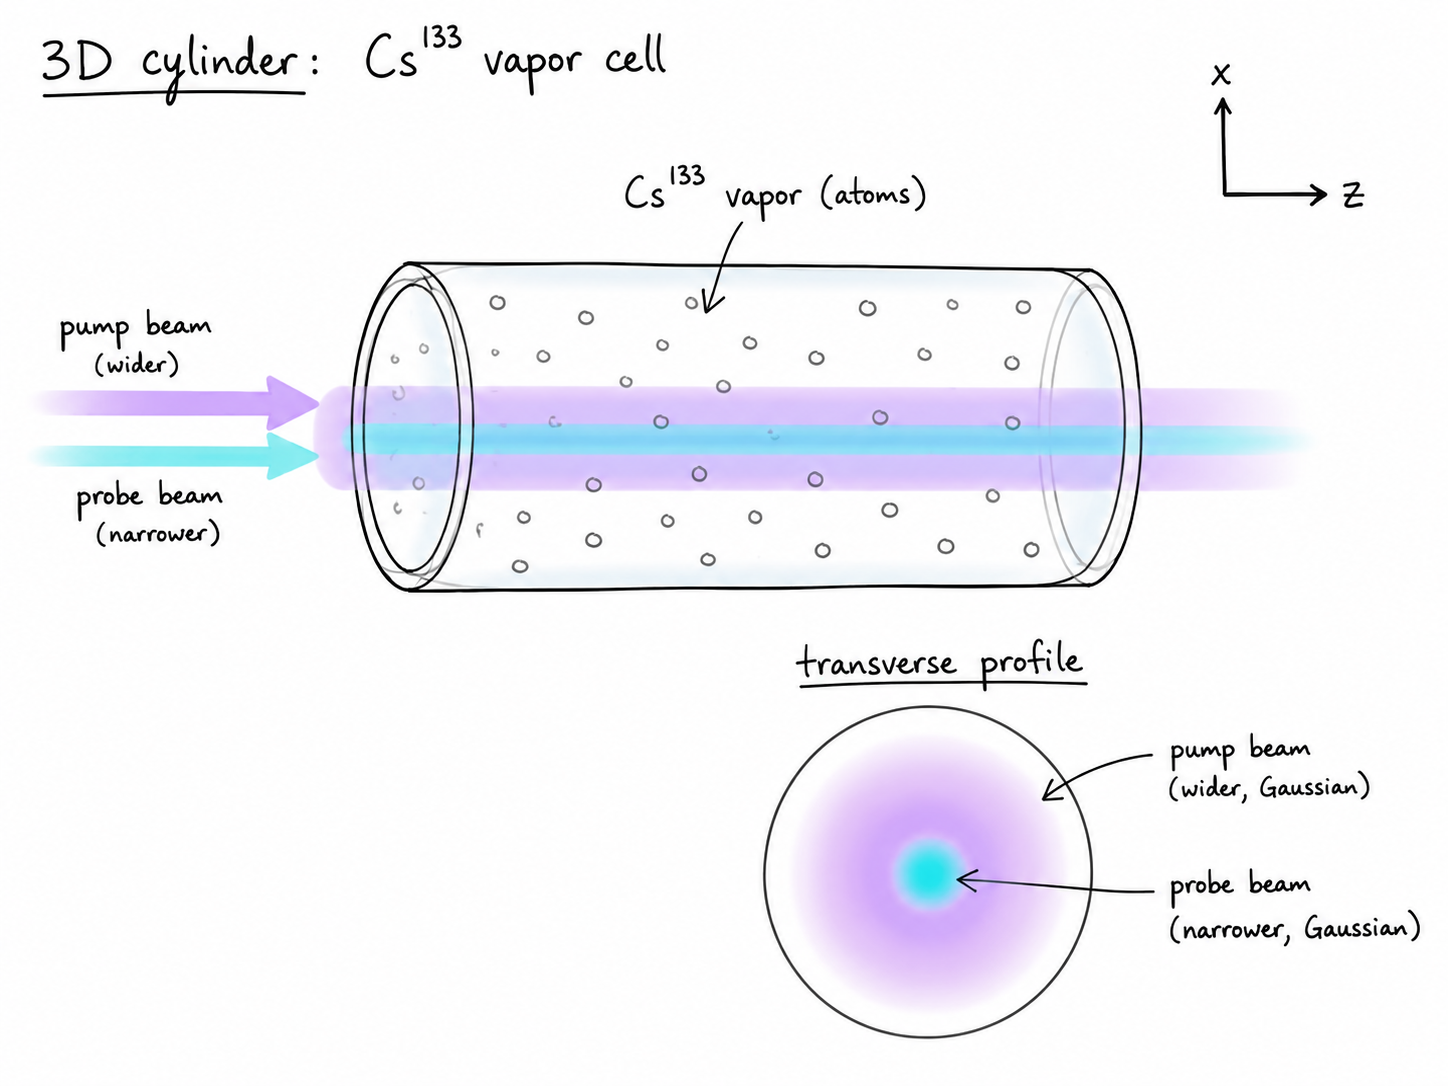
\includegraphics[width=0.72\textwidth]{Figures/ensemble_schematic.jpeg}
    \caption{Schematic representation of the reference warm-vapour geometry. The signal and control beams define a small optical interaction region inside the larger cylindrical vapour cell.}
    \label{fig:ensemble_schematic}
\end{figure}

This reference system is used as a validation case. The expected physical trends are already known: stronger confinement by buffer gas should slow motional loss, larger beams should increase the interaction time, magnetic-field gradients should produce phase dephasing, and phase mismatch should reduce directional retrieval. In this chapter, these expected trends are used to test whether the simulated quantity \(\mathcal{R}_{\mathrm{fib}}(t)\) behaves as a retrievable spin-wave mode.

\section{Directional Collective Emission}
\label{sec:results_directional_collective_emission}

The first validation test is the far-field emission pattern. During retrieval, the stored spin wave is converted into an optical polarization by the read control field. Each atom then contributes a small field amplitude, but the useful emission is not the incoherent sum of the emitted powers. It is the coherent sum of the fields. The direction in which these fields add constructively is fixed by the phase-matching condition~\cite{PsiL-odamIFm_GorshkovEtAl_2007},
\begin{equation}
    \mathbf{k}_{\mathrm{out}}
    =
    \mathbf{k}_{\mathrm{sig}}^{\mathrm{write}}
    -
    \mathbf{k}_{\mathrm{c}}^{\mathrm{write}}
    +
    \mathbf{k}_{\mathrm{c}}^{\mathrm{read}},
    \label{eq:results_phase_matching}
\end{equation}
where \(\mathbf{k}_{\mathrm{out}}\) is the retrieved optical wave vector, \(\mathbf{k}_{\mathrm{sig}}^{\mathrm{write}}\) is the signal wave vector during storage, and \(\mathbf{k}_{\mathrm{c}}^{\mathrm{write}}\) and \(\mathbf{k}_{\mathrm{c}}^{\mathrm{read}}\) are the write and read control-field wave vectors.

Figure~\ref{fig:far_field_angular_emission_profile} shows the simulated far-field angular distribution. The strongest emission is concentrated around the forward, phase-matched direction. This result is important because it confirms that the model is not simply tracking atomic survival. It is computing a collective interference pattern. The noise away from the central direction corresponds to residual constructive interference into other angular modes, but the dominant peak remains aligned with the expected retrieval direction.

\begin{figure}[htbp]
    \centering
    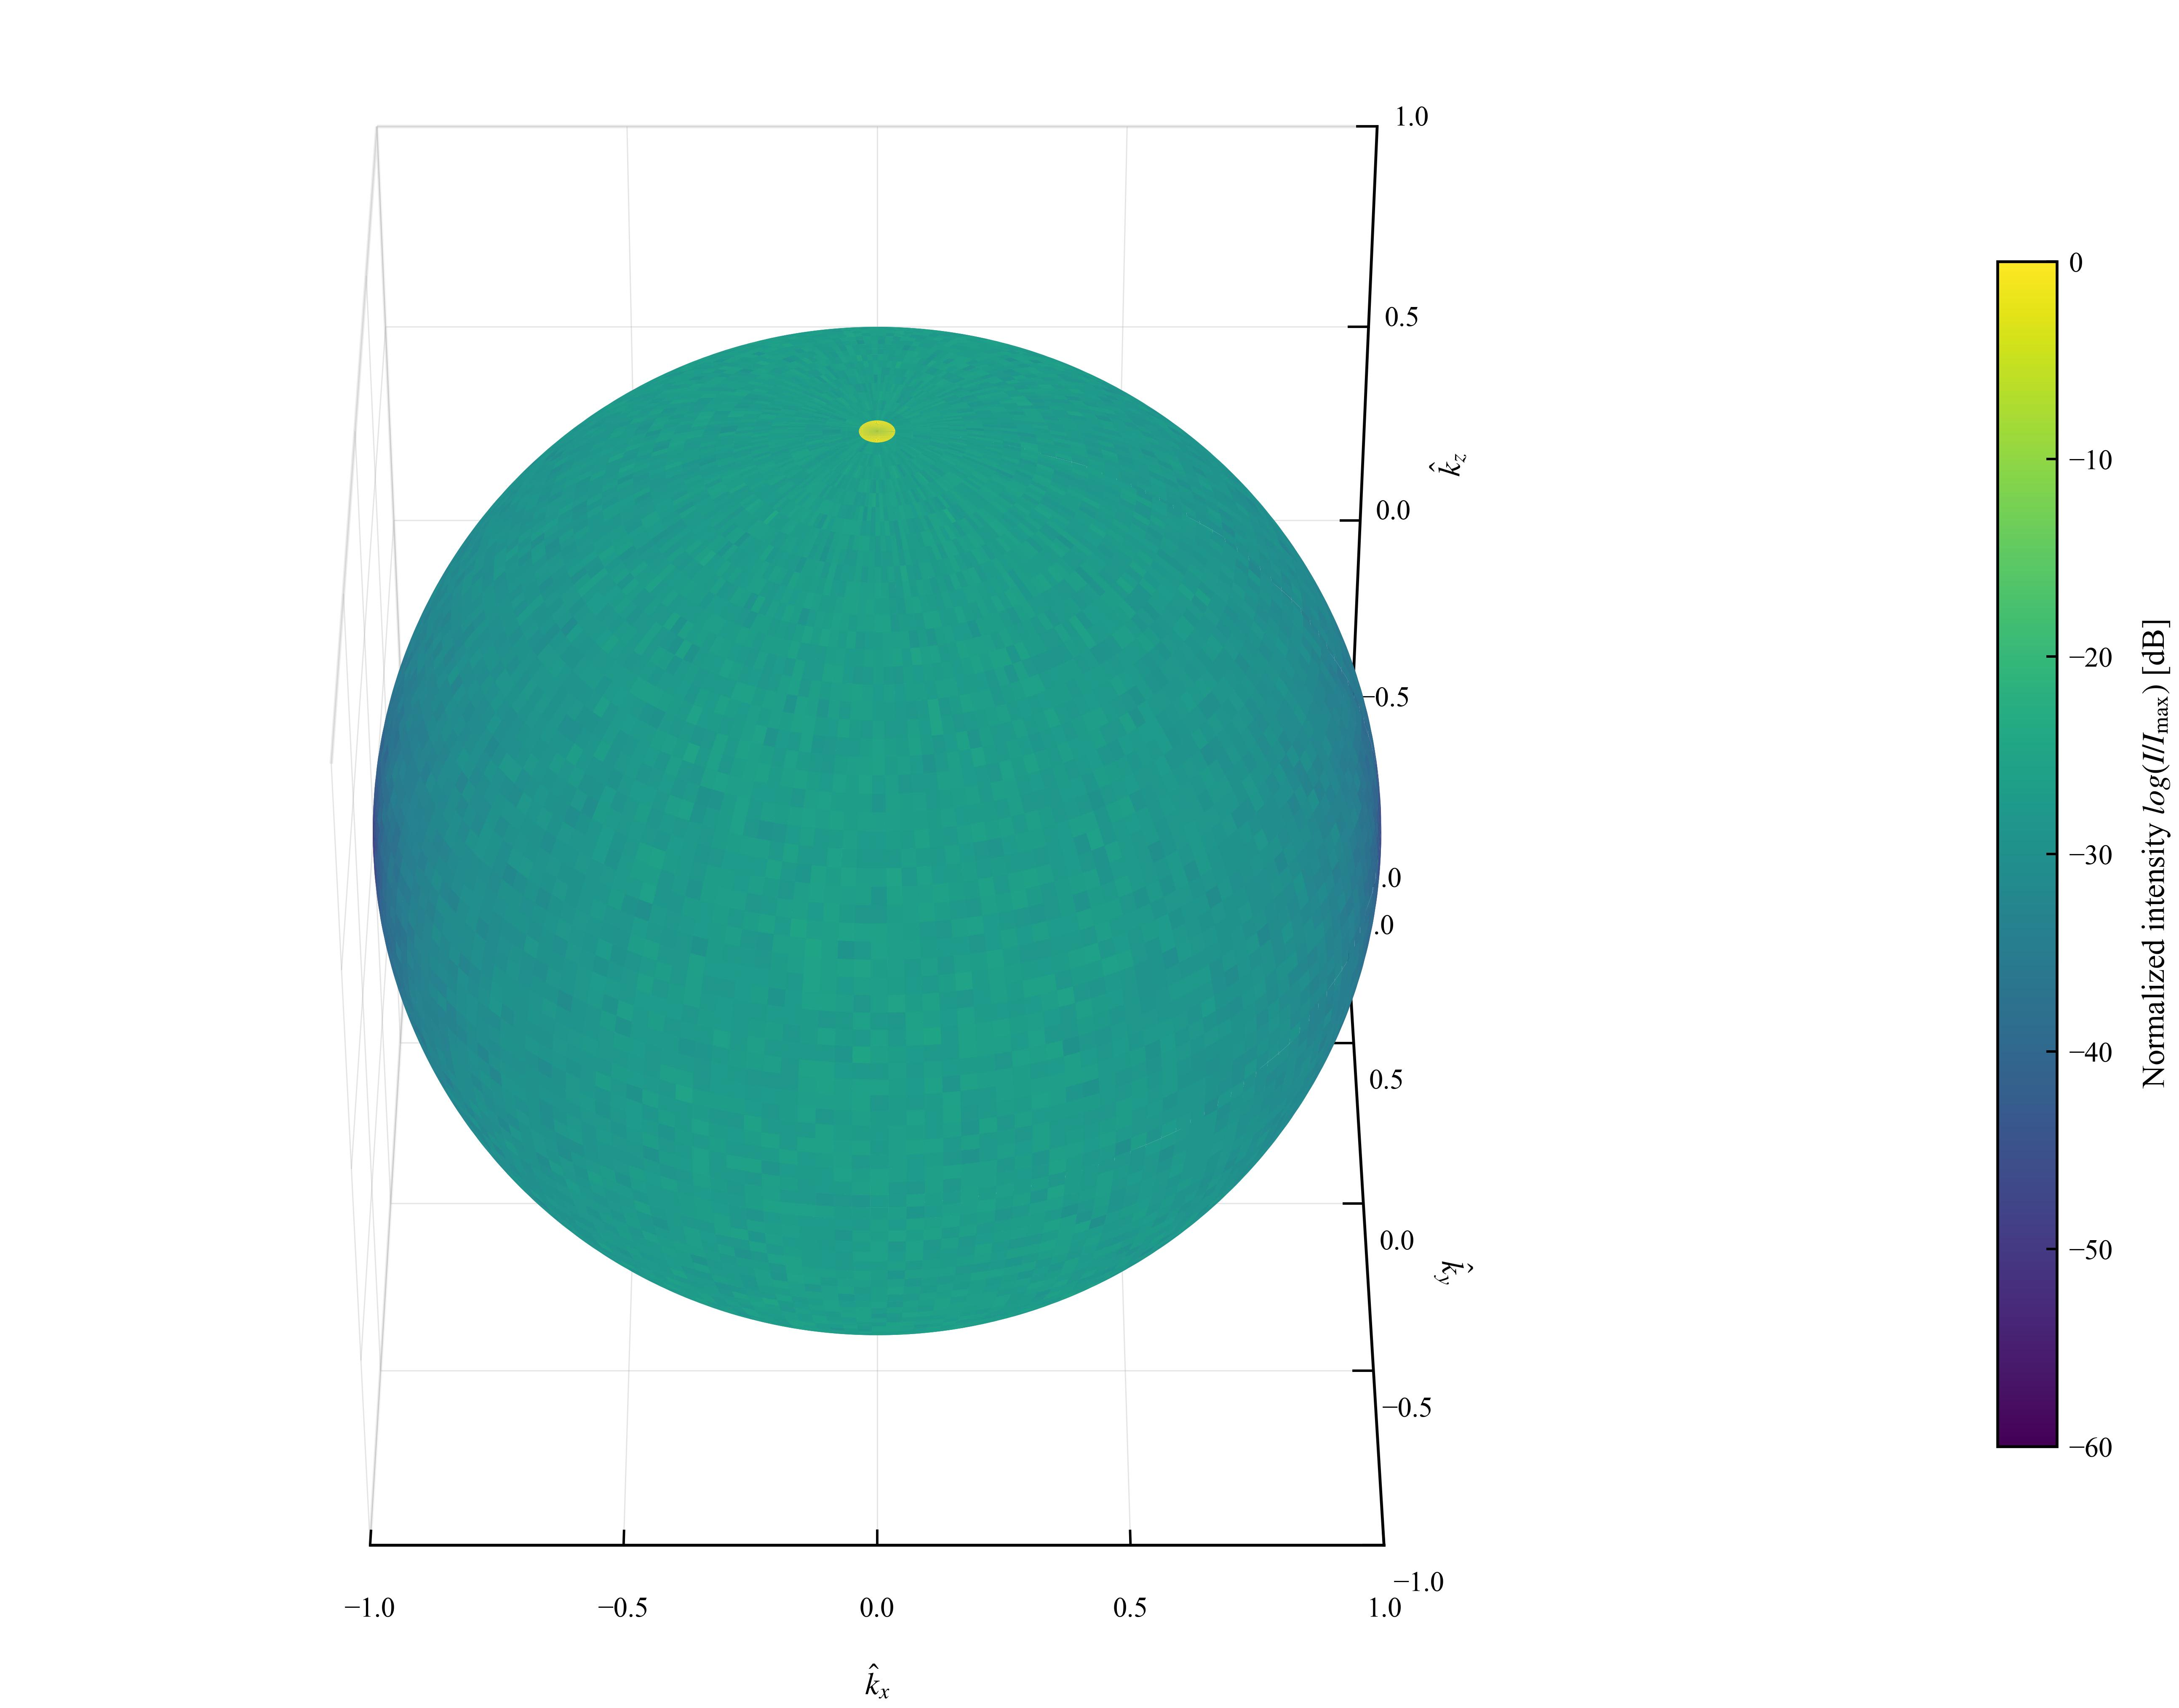
\includegraphics[width=0.70\textwidth]{Figures/far_field_angular_emission_profile.jpeg}
    \caption{Far-field angular emission profile obtained from the coherent dipole sum. The strongest emission appears in the forward phase-matched direction, validating that the simulated spin wave produces directional collective retrieval.}
    \label{fig:far_field_angular_emission_profile}
\end{figure}

The physical meaning of this result is simple. If the atomic phases are arranged according to the written spin wave, the emitted fields add in the direction selected by Eq.~\eqref{eq:results_phase_matching}. If the phases are randomized, the same atoms may still emit light, but the fields no longer add into the selected mode. Directional emission is therefore the first signature that the simulated observable is sensitive to the collective mode structure.

\section{Monte Carlo Convergence}
\label{sec:results_monte_carlo_convergence}

The second validation test concerns numerical convergence. Since the simulation samples a finite number of atoms and stochastic trajectories, the retrieved signal must be shown not to be dominated by rare events or sampling noise. For this reason, repeated Monte Carlo realizations are compared with the ensemble mean.

\begin{figure}[htbp]
    \centering
    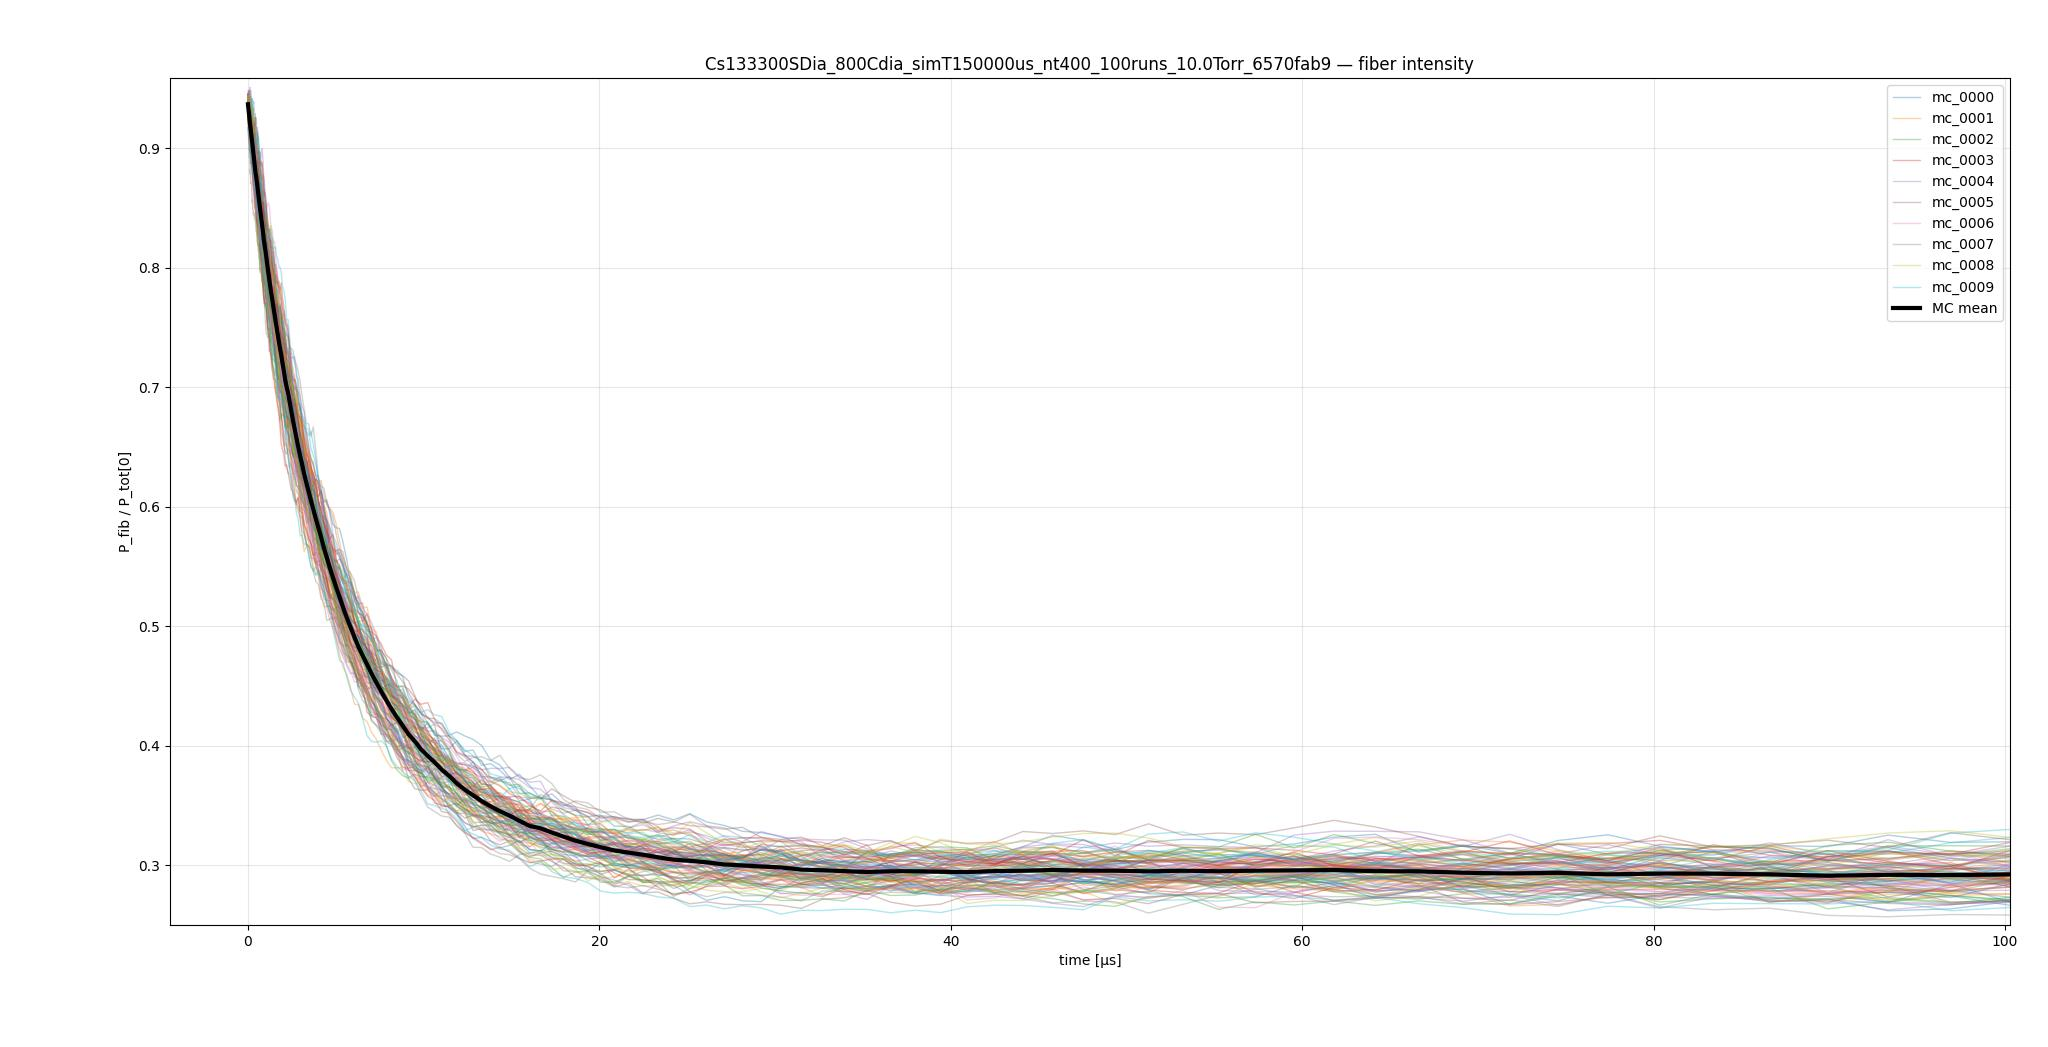
\includegraphics[width=0.72\textwidth]{Figures/monte_carlo_convergence.jpeg}
    \caption{Monte Carlo convergence of the normalized retrieved signal. Individual stochastic realizations follow the same global decay trend as the ensemble mean, showing that the simulated decay is not dominated by a small number of rare trajectories.}
    \label{fig:monte_carlo_convergence}
\end{figure}

Figure~\ref{fig:monte_carlo_convergence} shows that different realizations fluctuate around the same decay curve. The fluctuations are expected because the atoms follow different random trajectories, but the mean behaviour is stable. This validates the use of the Monte Carlo average as a numerical estimator of the retrieval-mode decay. The standard uncertainty of a simple Monte Carlo average decreases as the inverse square root of the number of independent samples~\cite{MonteCarloNotes}. Increasing the number of simulated atoms therefore improves the smoothness of the retrieved decay curve, but does not change the physical trend once convergence has been reached.

\section{Gas-Phase Transport and Buffer-Gas Pressure}
\label{sec:results_buffer_gas_pressure}

After the collective emission and numerical convergence have been validated, the first physical parameter scan is the buffer-gas pressure. Buffer gas changes the motion of alkali atoms by producing frequent velocity-changing collisions. In a warm vapour without sufficient confinement, atoms carrying the spin-wave coherence leave the high-overlap optical mode on a transit-time scale. Once they leave this region, their contribution to \(P_{\mathrm{fib}}(t)\) is reduced even if their internal ground-state coherence has not been completely destroyed.

The diffusion model captures this effect through the diffusion coefficient \(D\). Larger buffer-gas pressure reduces the diffusion coefficient and therefore slows the spatial escape of atoms from the signal and control beam volume. The expected result is a slower decay of \(\mathcal{R}_{\mathrm{fib}}(t)\).

\begin{figure}[htbp]
    \centering
    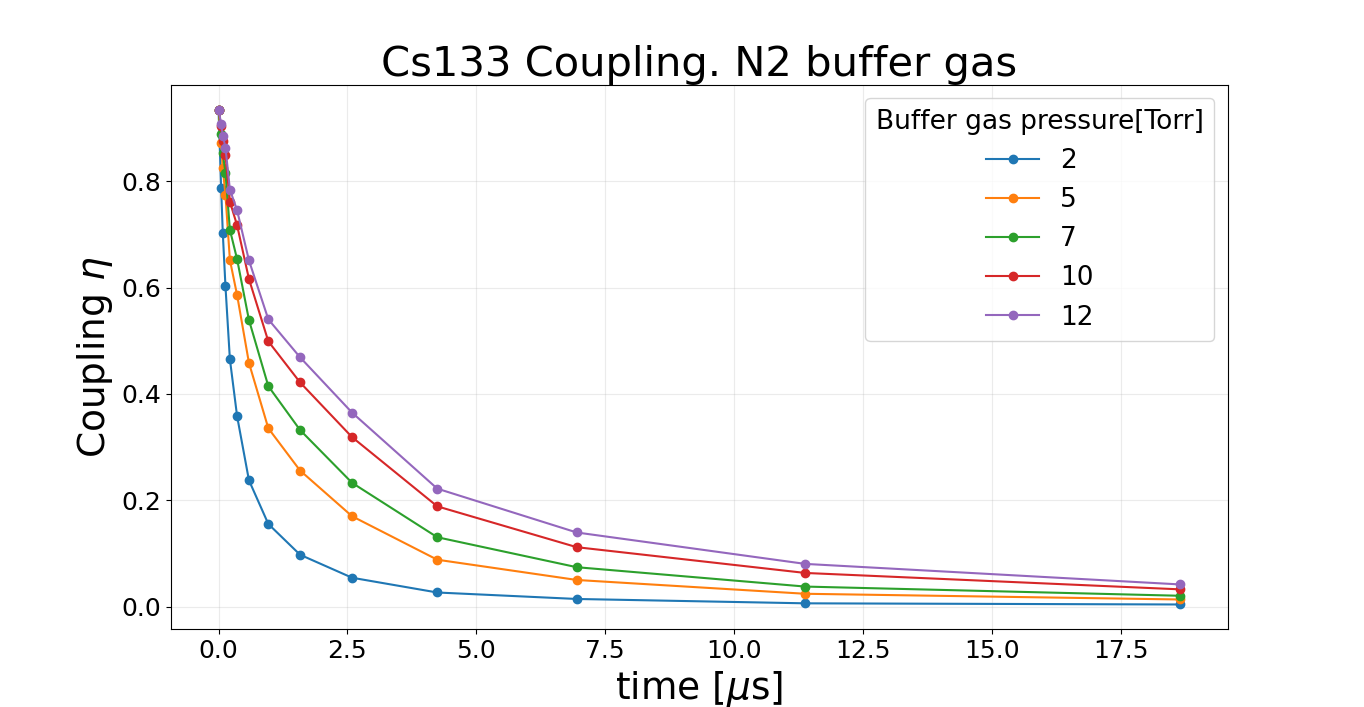
\includegraphics[width=0.72\textwidth]{Figures/pressure_scan_coupling_decay.jpeg}
    \caption{Pressure scan of the normalized fibre-coupled retrieval. Increasing the buffer-gas pressure reduces atomic diffusion and extends the time over which atoms remain inside the high-overlap optical mode.}
    \label{fig:pressure_scan_coupling_decay}
\end{figure}

Figure~\ref{fig:pressure_scan_coupling_decay} shows this behaviour. At lower pressure, the retrieval decays more rapidly because atoms diffuse away from the spatial region where the stored spin wave overlaps well with the readout mode. At higher pressure, the motion is slowed, and the collective mode survives for a longer time. The result should be interpreted as a mode-overlap effect. The atoms are not necessarily destroyed when they leave the beam. Rather, their phase and position no longer match the mode that can radiate efficiently back into the fibre.

\section{Beam-Size Dependence}
\label{sec:results_beam_size}

The same physical mechanism can be tested by changing the optical beam sizes. A larger beam defines a larger interaction region. An atom must move farther before its contribution to the signal-control overlap becomes small. Thus, increasing the signal or control beam size should increase the decay time of the retrieved mode.

\begin{figure}[htbp]
    \centering
    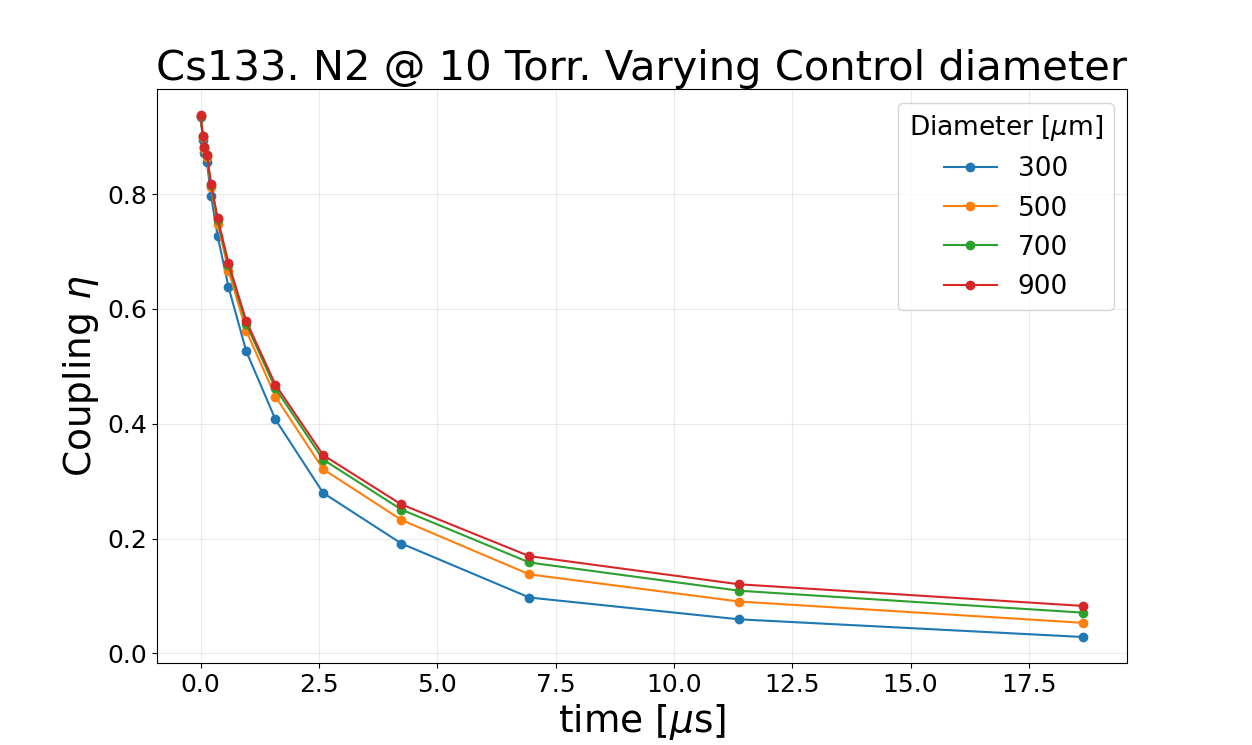
\includegraphics[width=0.72\textwidth]{Figures/beam_size_scan_coupling_decay.jpeg}
    \caption{Beam-size dependence of the normalized retrieval. Larger signal or control beams increase the spatial region over which atoms remain coupled to the readout mode, leading to a slower decay of \(P_{\mathrm{fib}}(t)/P_{\text{tot}}(0)\).}
    \label{fig:beam_size_scan_coupling_decay}
\end{figure}

Figure~\ref{fig:beam_size_scan_coupling_decay} confirms this trend. Larger beams give a longer coupling time because the stored spin wave is distributed over a wider transverse region. The decay is therefore less sensitive to short diffusive displacements. This result is consistent with the usual warm-vapour intuition that transit-time broadening is reduced when the optical mode is enlarged~\cite{Apgteitiav_FinkelsteinEtAl_2023}.

However, this improvement is not a free optimization. In an experiment, increasing the beam size can reduce optical intensity for fixed power, modify the EIT bandwidth, and change the optical depth sampled by the mode. These effects are not fully included in the present simulation. The result here should therefore be read as a statement about spatial mode survival: for fixed optical preparation, a larger beam makes the retrievable spin-wave mode less sensitive to atomic motion.

\section{Comparison with a Cold Gaussian Ensemble}
\label{sec:results_bec_comparison}

The same beam-size logic was also tested in a cold Gaussian ensemble. The simulated cloud contains \(10^8\) atoms with a Gaussian spatial distribution of width approximately \(\SI{1}{\milli\metre}\). The control and signal beams are taken to be smaller than the cloud, so that the stored mode is still defined by the optical overlap rather than by the full atom distribution.

\begin{figure}[htbp]
    \centering
    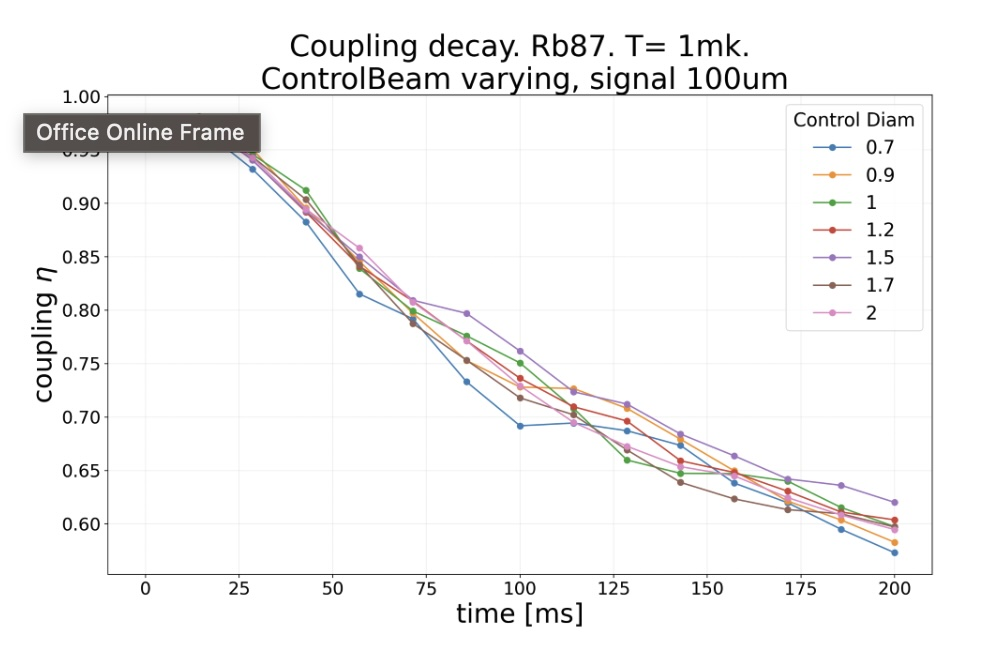
\includegraphics[width=0.72\textwidth]{Figures/bec_beam_size_scan.jpeg}
    \caption{Beam-size scan for a cold Gaussian ensemble. The same qualitative increase in coupling time is observed when the optical mode is enlarged, although the effect is weaker than in the warm-vapour reference case because thermal diffusion is no longer the dominant limitation.}
    \label{fig:bec_beam_size_scan}
\end{figure}

Figure~\ref{fig:bec_beam_size_scan} shows that increasing the beam size also increases the coupling time in the cold-cloud case, but the change is less pronounced than in the warm-vapour cell. This is expected. In the warm vapour, atoms move rapidly through the optical mode, so the transverse beam size directly controls the escape time. In the cold ensemble, the motion is slower and the dominant limitation is no longer the same diffusive transit through the beam. The result is useful because it shows that the same retrieval-overlap formalism can be applied to different atomic platforms, while the dominant physical mechanism changes.

\section{Geometric Phase Mismatch from Control-Beam Angle}
\label{sec:results_control_beam_angle}

A change in the relative angle between the signal and control fields changes the spin-wave wave vector,
\begin{equation}
    \Delta\mathbf{k}
    =
    \mathbf{k}_{\mathrm{sig}}
    -
    \mathbf{k}_{\mathrm{c}},
    \label{eq:results_delta_k_angle}
\end{equation}
where \(\mathbf{k}_{\mathrm{sig}}\) and \(\mathbf{k}_{\mathrm{c}}\) are the signal and control wave vectors during storage. Even a small angular mismatch introduces a transverse spin-wave phase gradient. This matters because atoms that move transversely through this phase grating accumulate different phases. If the spin-wave period is short, a small displacement is enough to change the phase significantly. If the spin-wave period is long, the same displacement produces a smaller phase error.

\begin{figure}[htbp]
    \centering
    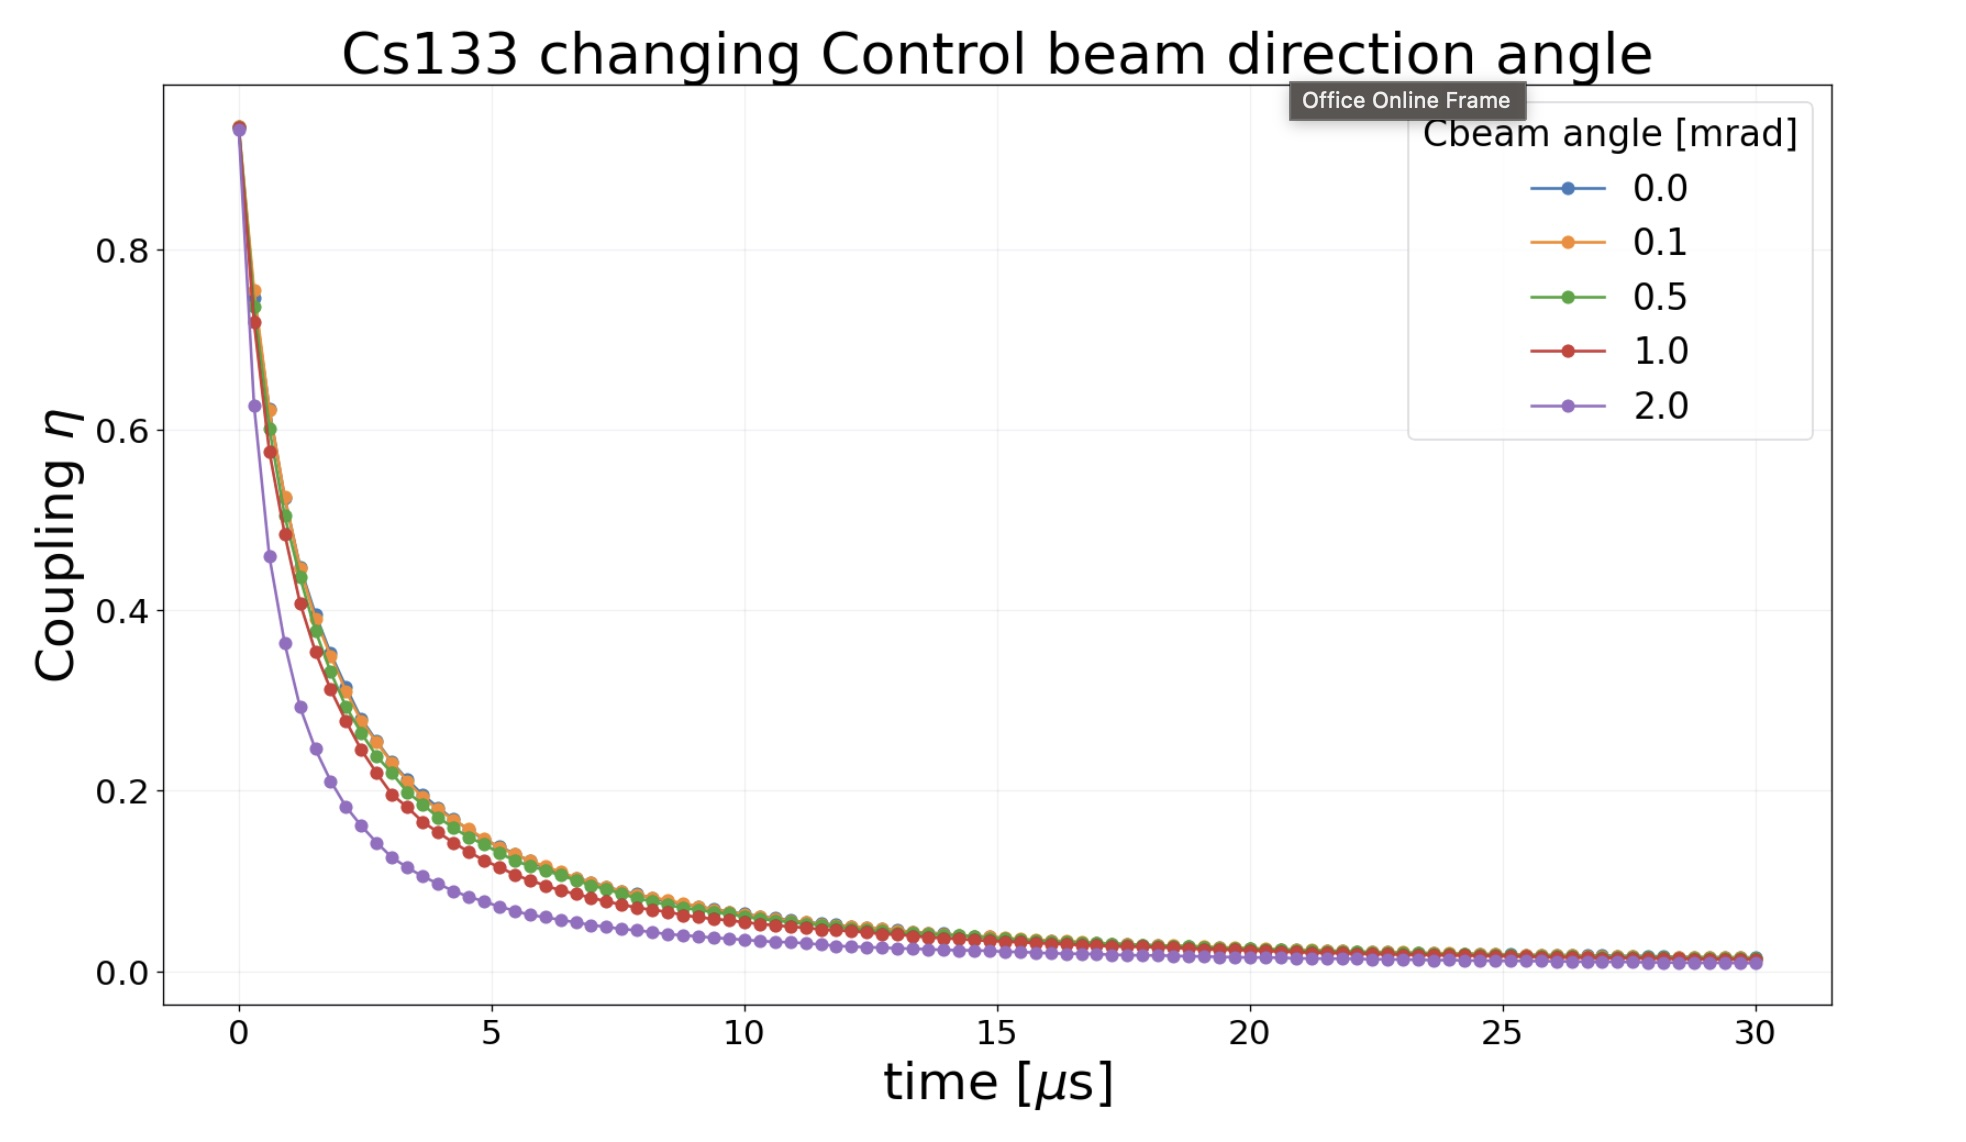
\includegraphics[width=0.72\textwidth]{Figures/control_beam_angle_scan.jpeg}
    \caption{Control-beam angle scan. Changing the signal-control angle modifies the spin-wave wave vector and therefore the sensitivity of the stored coherence to atomic motion.}
    \label{fig:control_beam_angle_scan}
\end{figure}

Figure~\ref{fig:control_beam_angle_scan} shows the effect of this geometric phase mismatch. The retrieved mode decays faster when the spin-wave phase varies more rapidly across the ensemble. This is not a loss of atoms; it is a loss of relative phase. The atoms can still carry ground-state coherence, but the spatial phase pattern no longer matches the phase-matched readout mode.

This result is especially important for warm-vapour EIT, where signal and control beams are usually kept nearly co-propagating. Small relative angles can broaden the two-photon resonance and introduce motional dephasing because the effective two-photon wave vector becomes nonzero~\cite{Apgteitiav_FinkelsteinEtAl_2023}. The simulation reproduces this intuition at the level of the retrievable spin-wave mode.

\section{Magnetic-Gradient Dephasing}
\label{sec:results_magnetic_gradient}

A magnetic-field gradient provides a different way to destroy the collective mode. Instead of changing the optical phase written into the spin wave, it makes the ground-state splitting position dependent. The accumulated phase of atom \(j\) may be written as
\begin{equation}
    \phi_j(t)
    =
    \int_0^t
    \omega_{sg}\!\left(\mathbf{r}_j(t')\right)
    \,dt',
    \label{eq:results_magnetic_phase}
\end{equation}
where \(\omega_{sg}(\mathbf{r})\) is the local angular frequency splitting between \(\ket{g}\) and \(\ket{s}\), and \(t'\) is the integration variable. If \(\omega_{sg}\) is the same everywhere, all atoms acquire the same phase and the collective interference is unchanged. If \(\omega_{sg}\) varies across the cell, different atoms acquire different phases, and the collective readout is reduced.

\begin{figure}[htbp]
    \centering
    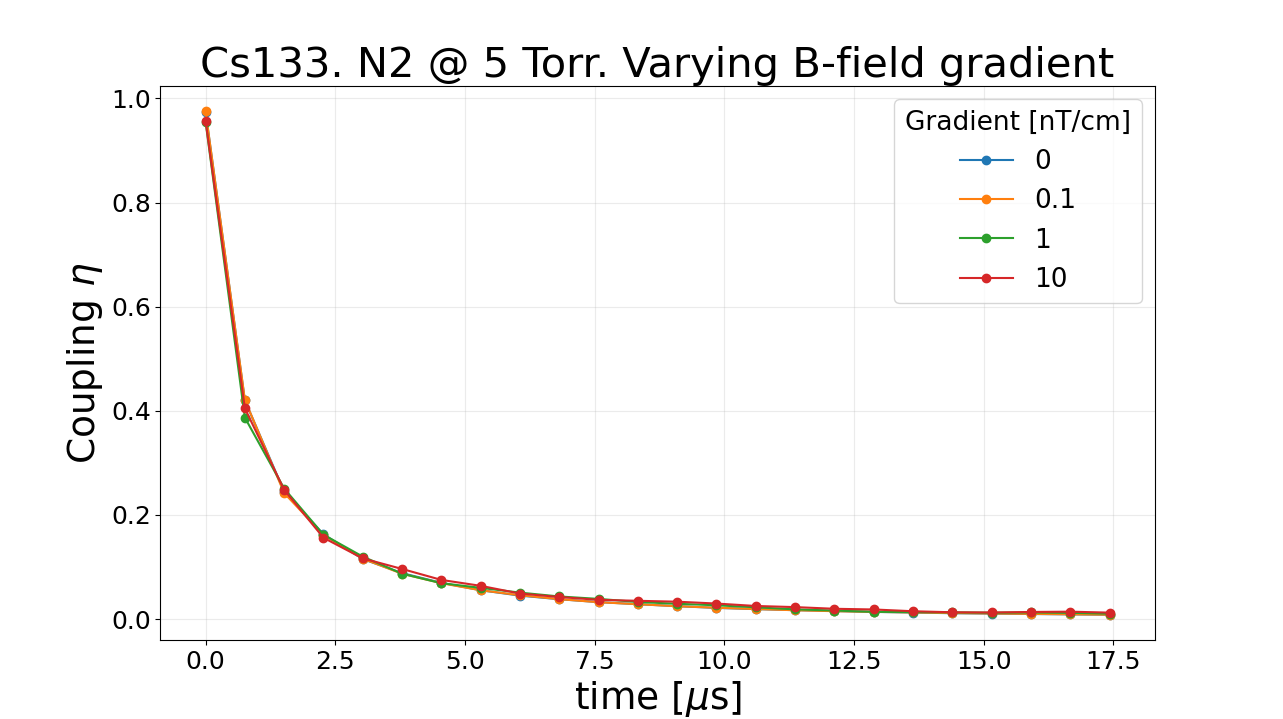
\includegraphics[width=0.72\textwidth]{Figures/magnetic_gradient_scan.jpeg}
    \caption{Magnetic-gradient-induced decay of the normalized retrieval. A spatially varying ground-state splitting causes atoms in different parts of the ensemble to accumulate different phases, reducing constructive retrieval into the target mode.}
    \label{fig:magnetic_gradient_scan}
\end{figure}

Figure~\ref{fig:magnetic_gradient_scan} shows that increasing the magnetic gradient accelerates the decay of \(P_{\mathrm{fib}}(t)/P_{\text{tot}}(0)\). The physical mechanism is phase scrambling. Unlike beam-size loss, where atoms leave the optical mode, magnetic dephasing can reduce retrieval even when the atoms remain inside the beam. This distinction is useful experimentally because the two mechanisms require different improvements. Beam-size or buffer-gas changes address spatial escape, while magnetic shielding and field homogeneity address phase evolution.

\section{Compact-Cell Geometry}
\label{sec:results_compact_cell_geometry}

The reference cell is long compared with its optical mode and has a diameter much larger than the beam waist. In that regime, atoms can diffuse out of the optical mode before wall collisions dominate the retrieval decay. The compact geometry changes this balance. The simulated compact cell has diameter \(\SI{1}{\milli\metre}\) and length \(\SI{10}{\milli\metre}\), with control and signal FWHM diameters of approximately \(\SI{0.8}{\milli\metre}\) and \(\SI{0.3}{\milli\metre}\), respectively. The optical mode now occupies a substantial fraction of the cell cross-section.

This changes the interpretation of the decay. In the reference geometry, an atom can leave the optical mode while still being far from the cell boundary. In the compact geometry, the cell wall is close to the optical mode. Atoms that carry the spin-wave coherence therefore reach the wall on timescales relevant for the simulated retrieval decay. The boundary condition can no longer be ignored.

\section{Wall Coatings as an Effective Boundary Condition}
\label{sec:results_wall_coatings}

The wall interaction has two parts that must be kept conceptually separate. The first is mechanical reflection: the atom remains inside the cell after hitting the boundary. The second is internal-state survival: the atom may or may not retain the ground-state coherence that allows it to contribute to the spin wave. These two processes are not the same. An atom can return to the vapour mechanically while its spin coherence has already been randomized by the surface interaction~\cite{OP_Happer_1972}.

The simulation represents the coating as an effective survival probability per wall collision. If \(N_{\text{b}}\) is the average number of wall collisions before depolarization, the survival probability per collision is written as
\begin{equation}
    p_{\mathrm{survive}}
    =
    1-\frac{1}{N_{\text{b}}},
    \label{eq:results_wall_survival_probability}
\end{equation}
where \(p_{\mathrm{survive}}\) is the probability that the atomic ground-state coherence survives one wall encounter. This model does not describe the microscopic chemistry of the coating. Instead, it condenses the complicated surface interaction into a single effective parameter.

Anti-relaxation coatings are useful because they reduce the probability that a wall encounter destroys the atomic spin state. The detailed coating performance depends on material, temperature, surface coverage, adsorption dynamics, and morphology~\cite{Aiacoavc_ChiEtAl_2020}. For the compact-cell simulations, this complexity is represented by scanning \(N_{\text{b}}\). Small \(N_{\text{b}}\) corresponds to a poor coating or nearly depolarizing wall. Large \(N_{\text{b}}\) corresponds to a wall that preserves coherence over many collisions.

\begin{figure}[htbp]
    \centering
    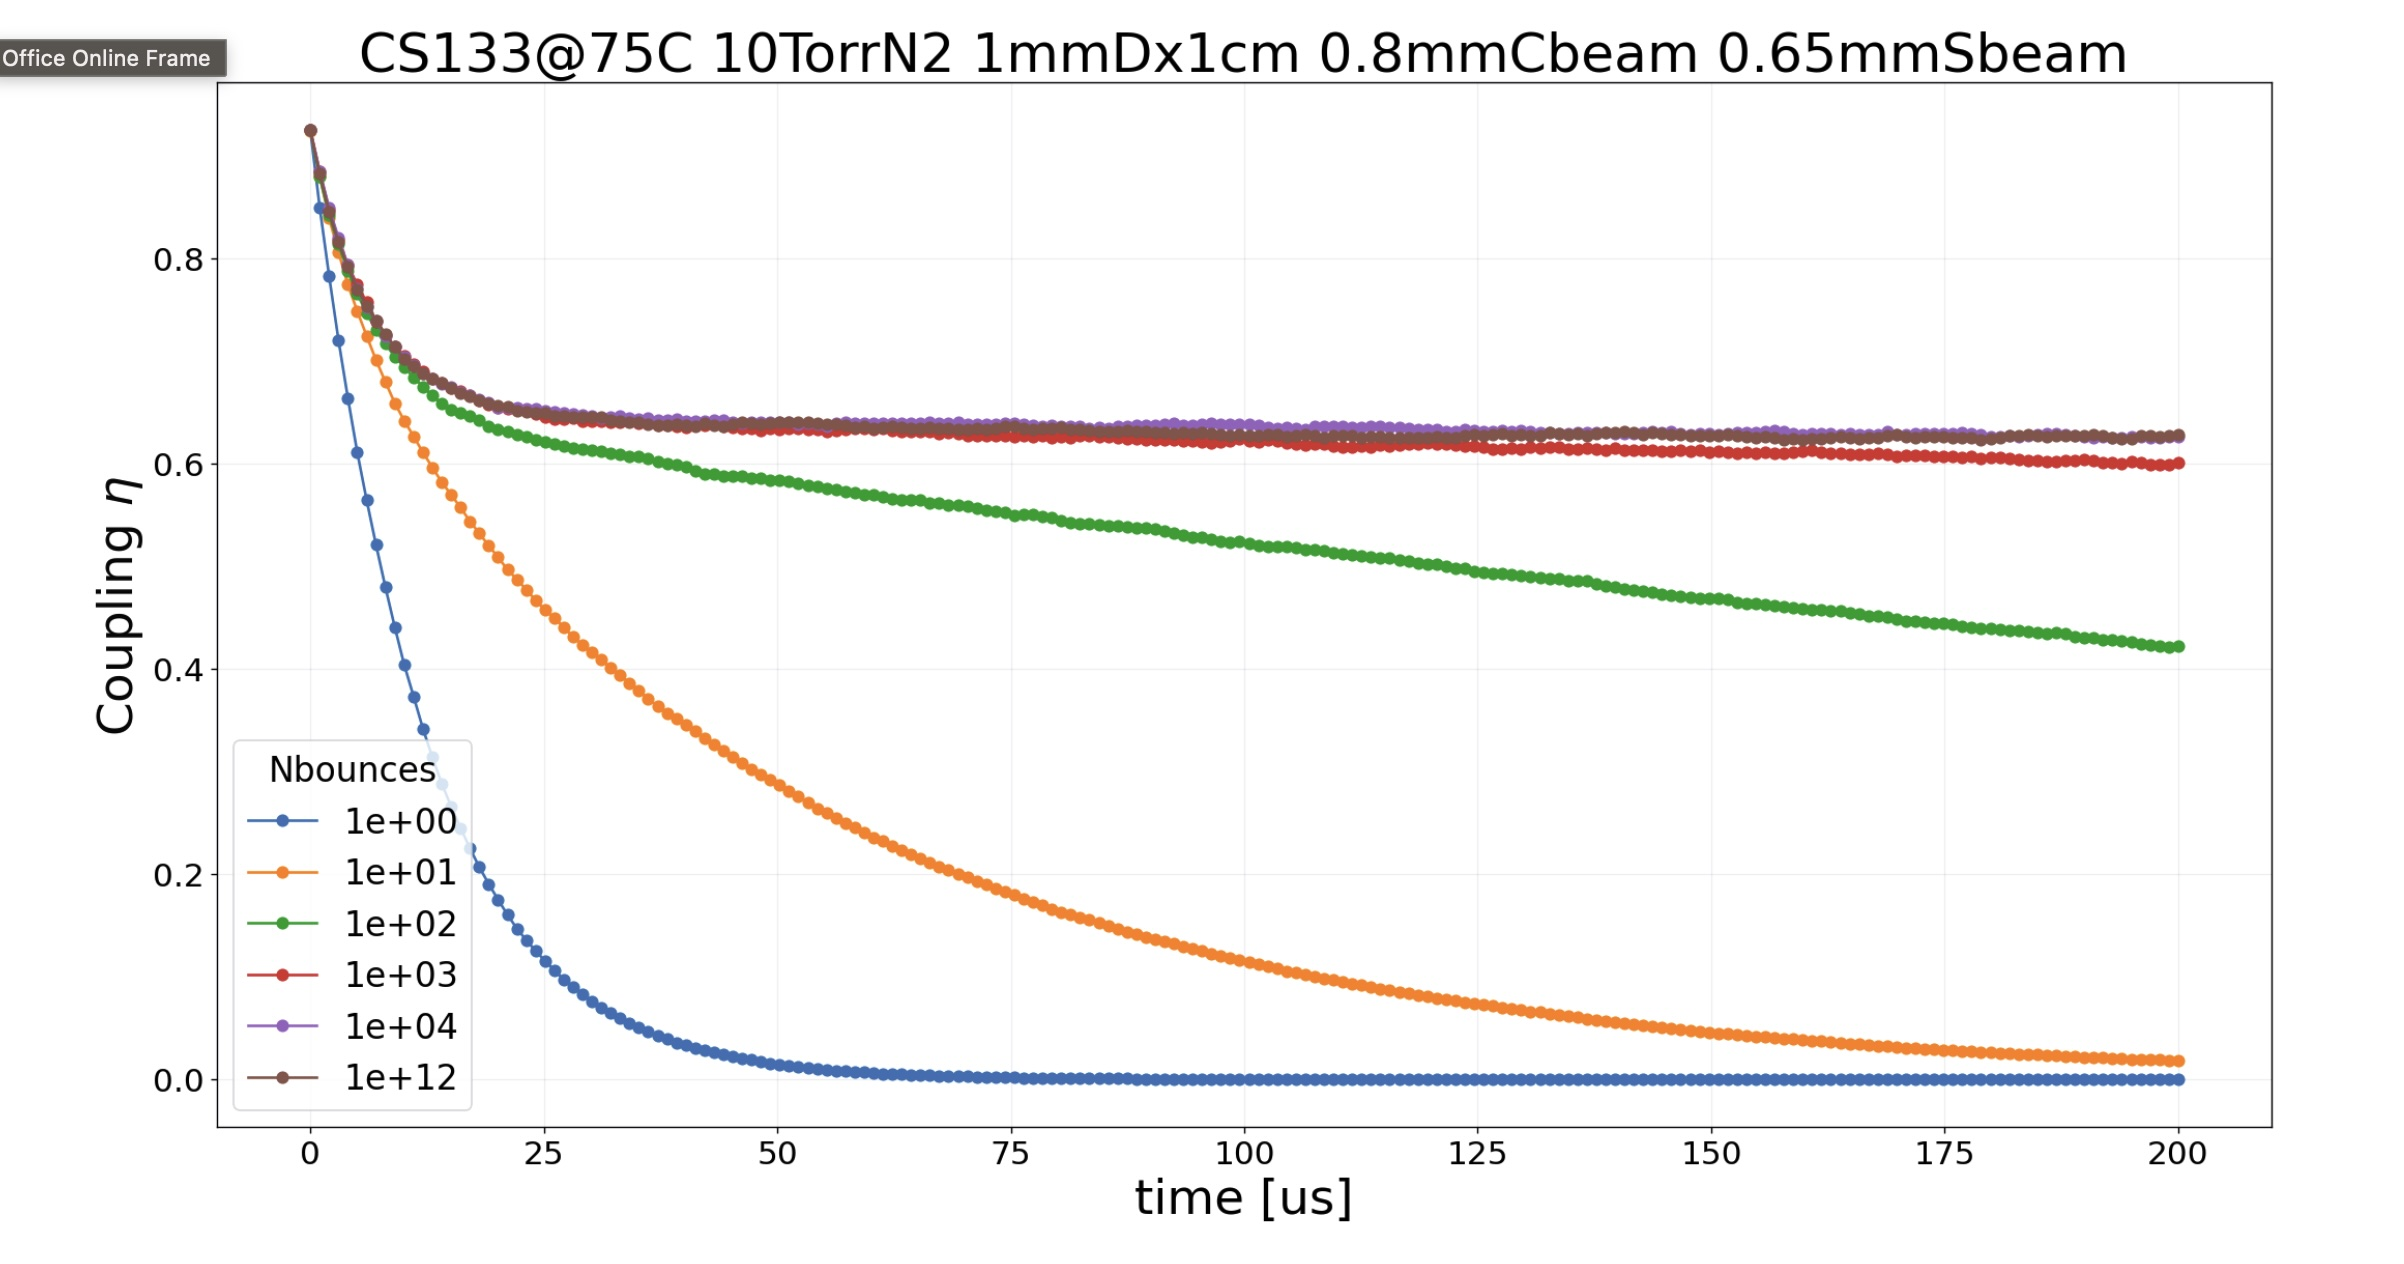
\includegraphics[width=0.72\textwidth]{Figures/coating_bounce_scan.jpeg}
    \caption{Compact-cell coating scan. Increasing the average number of coherence-preserving wall collisions \(N_{\text{b}}\) improves the retrieval decay when wall relaxation is the dominant loss channel.}
    \label{fig:coating_bounce_scan}
\end{figure}

Figure~\ref{fig:coating_bounce_scan} shows that increasing \(N_{\text{b}}\) improves the retrieval lifetime for poor coatings. In this regime, each wall encounter has a significant probability of removing the atom from the collective spin wave, so wall collisions act almost like an absorbing boundary for the retrievable mode. When \(N_{\text{b}}\) is increased, atoms can hit the wall and return to the vapour while still carrying coherence. The retrieved signal therefore decays more slowly.

The improvement does not continue indefinitely. Once \(N_{\text{b}}\) is large enough, the curves begin to converge. In that regime, wall-induced depolarization is no longer the dominant limitation. The remaining decay is set mainly by diffusion through the optical mode, the finite cell geometry, and imperfect overlap with the readout mode. This saturation is an important design result: beyond a certain coating quality, improving the wall survival alone does not strongly increase \(P_{\mathrm{fib}}(t)/P_{\text{tot}}(0)\).

\section{Temperature Dependence in the Compact Cell}
\label{sec:results_temperature_compact_cell}

Temperature affects a warm-vapour memory in two opposite ways. Increasing the temperature raises the alkali vapour pressure and can increase the optical depth, which is beneficial for storage and retrieval efficiency. At the same time, higher temperature increases the thermal velocity and modifies the transport through the buffer gas. It can also make wall interactions and coating stability more important~\cite{Apgteitiav_FinkelsteinEtAl_2023,Aiacoavc_ChiEtAl_2020}.

The present simulation focuses on the transport and mode-overlap side of this trade-off. It does not compute the full temperature dependence of the EIT optical depth. Therefore, the temperature scan should not be read as a complete optimization of memory efficiency. It should be read as a test of how motion and wall encounters affect the retrievable spin-wave mode under different thermal conditions.

\begin{figure}[htbp]
    \centering
    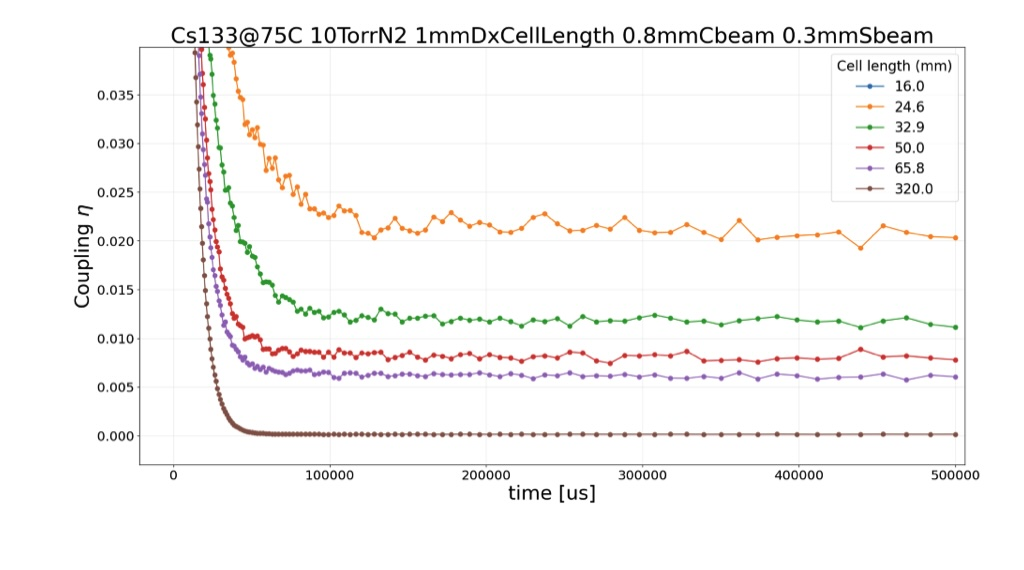
\includegraphics[width=0.72\textwidth]{Figures/compact_temperature_scan.jpeg}
    \caption{Temperature dependence of the compact-cell retrieval for different wall-survival parameters. The plotted decay reflects the transport and wall-relaxation contribution to the retrievable-mode lifetime, not the full optical-depth optimization of an EIT memory.}
    \label{fig:compact_temperature_scan}
\end{figure}

Figure~\ref{fig:compact_temperature_scan} shows the resulting temperature-dependent retrieval decay. When the wall survival is low, the decay is strongly affected by the rate at which atoms reach the boundary. When the wall survival is high, the decay becomes less sensitive to the coating parameter and more sensitive to residual mode-overlap loss. This is the regime in which atoms may survive wall encounters but still fail to return with the correct spatial phase and optical overlap for efficient fibre-coupled retrieval.

\section{Cell Length and Spin-Wave Phase}
\label{sec:results_cell_length_spin_wave}

The compact-cell geometry also makes the relationship between cell length and spin-wave phase important. The stored spin wave contains a phase factor
\begin{equation}
    e^{i\Delta\mathbf{k}\cdot\mathbf{r}},
    \label{eq:results_spin_wave_phase_factor}
\end{equation}
where \(\Delta\mathbf{k}\) is set by the signal-control geometry. If the cell length is short compared with the spin-wave period, the phase does not vary strongly across the cell. If the cell spans many spin-wave periods, different longitudinal regions of the cell can contribute with very different phases.

\begin{figure}[htbp]
    \centering
    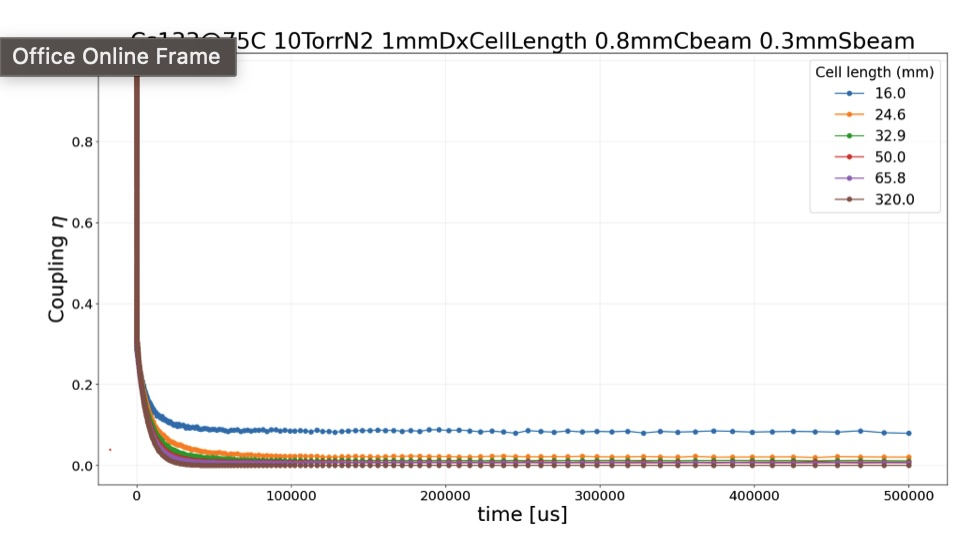
\includegraphics[width=0.72\textwidth]{Figures/cell_length_spin_wave_scan.jpeg}
    \caption{Cell-length scan relative to the spin-wave phase period. When the cell length spans many spin-wave periods, different parts of the ensemble contribute with different phases, reducing the retrievable collective mode.}
    \label{fig:cell_length_spin_wave_scan}
\end{figure}

Figure~\ref{fig:cell_length_spin_wave_scan} shows that the long-time plateau is sensitive to the relation between cell length and spin-wave phase. This result should not be interpreted as a simple volume effect. A longer cell contains more atoms, but it also samples more of the spin-wave phase pattern. If the phase varies significantly over the cell, the coherent sum into the target mode can decrease because different regions interfere less constructively.

This effect is especially relevant when comparing compact and elongated geometries. Miniaturization does not only change the wall-collision rate. It also changes how much of the spin-wave phase structure is sampled by the ensemble and how this structure overlaps with the readout mode.
